\documentclass[11pt]{article}

\usepackage[a4paper,margin=28mm]{geometry}
\usepackage{amsmath,amssymb,amsthm,mathtools}
\usepackage{mathrsfs}
\usepackage{tikz}
\usetikzlibrary{positioning}
\usepackage{microtype}
\usepackage{enumitem}
\usepackage[numbers,sort&compress]{natbib}
\usepackage[hidelinks]{hyperref}

\newtheorem{theorem}{Theorem}[section]
\newtheorem{proposition}[theorem]{Proposition}
\newtheorem{lemma}[theorem]{Lemma}
\newtheorem{corollary}[theorem]{Corollary}
\theoremstyle{definition}
\newtheorem{definition}[theorem]{Definition}
\theoremstyle{remark}
\newtheorem{remark}[theorem]{Remark}
\newtheorem{problem}[theorem]{Problem}

\newcommand{\Gtwo}{\mathcal G_2}
\newcommand{\Pred}{\operatorname{Pred}}
\newcommand{\Real}{\operatorname{Real}}
\newcommand{\Slice}{\mathsf{Slice}}
\newcommand{\VCbox}{\operatorname{VC}^{\Box}}
\newcommand{\FCP}{\mathrm{FCP}}
\newcommand{\eps}{\varepsilon}
\newcommand{\Vlive}{\mathcal V_{k,\mathrm{live}}}


\title{Higher-Arity VC Profiles of Candidate Rejection in Fixed-Interface Clause Systems}
\author{Takayuki Kuriyama}
\date{}

\begin{document}
\maketitle

\begin{abstract}
The learning algorithm of Shoudai, Matsumoto, Suzuki, and Uchida tests each
non-fact fixed-interface candidate clause by searching a Cartesian product of
residual substitutions indexed by its distinct variable labels.  We isolate
the pointwise Boolean candidate-rejection relation underlying this
body-positive/head-negative test and determine its higher-arity Cartesian-box
shattering profile.

Our main structural conclusion is that candidate rejection has two different
sharp information scales.  Once a target FICS \(\Gamma\) with at most \(m\)
clauses is fixed, only polynomially many bounded candidate syntaxes over its
active target predicates remain.
Hence, for every fixed \(1\le r\le k\),
\[
d_r(\Gamma)
=
O((\log(m+1))^{1/r}).
\]
This logarithmic scale is simultaneously sharp inside one target: for every
fixed \(k\ge2\) we construct a bounded family \(\Gamma_m^\star\) such that,
for all \(1\le r\le k\),
\[
d_r(\Gamma_m^\star)
=
\Theta_{k,r}((\log(m+1))^{1/r})
\]
at once, using live admissible candidates, and
\[
\log_2|\mathcal V_k(\Gamma_m^\star)|
=
\Theta_k(\log(m+1)).
\]
The construction stores all required labelings in finite banks of live
classifier predicates inside one master target and selects a labeling only by
varying the candidate head predicate.

At the global class level, where the target presentation may also vary, the
information scale increases by a factor of \(m\).  For every fixed bounded
FICS regime \(\mathfrak B\),
\[
d_r^{\mathfrak B}(m)
=
O_{\mathfrak B,k,r}((m\log(m+1))^{1/r}),
\]
and for every fixed \(k\ge2\) one bounded regime \(\mathfrak B_k\),
independent of \(m\) and \(r\), simultaneously attains the matching order for
all \(r\le k\), already in the live-candidate subclass.

The sharp lower bounds require more than finite-class counting.  We combine
fixed-length residual compression with a linear-size simulation of partial
DFAs by rank-two FICSs that preserves the finite context property.  Exact
length gates confine the rejection relation to the intended finite
substitution boxes, while explicit anchored contexts and ordered-boundary
positive examples expose the required predicate and residual representations.
At any update stage occurring after the corresponding finite exposure
threshold, Algorithm~3 literally enumerates the translated candidate and
tests the prescribed box.  This learner-side realization is conditional on
the occurrence of such an update stage.

Thus the candidate-rejection geometry separates a global \(m\log m\)
information regime, in which the target presentation also varies, from an
exact fixed-target \(\log m\) regime measuring variation in the target-induced
candidate class of one target.
\end{abstract}

\section{Introduction}

Learning graph languages requires controlling both the internal structure of
individual graph fragments and the ways in which several fragments interact
inside grammatical rules. Fixed-interface clause systems (FICSs), introduced
by Shoudai, Matsumoto, Suzuki, and Uchida, provide a logic-programming
framework in which such interactions are represented by graph-pattern clauses.
For bounded systems satisfying their finite context property (FCP), the
learner uses positive presentations and membership queries and admits bounded
candidate clauses by testing families of substitutions
\cite{ShoudaiEtAl2026}.

The product structure studied here is already explicit in that candidate test.
For a non-fact candidate \(\gamma\), let
\(X(\gamma)=\{x_1,\ldots,x_k\}\)
be the set of distinct variable labels.  The learner searches substitution
families indexed by this set, i.e. a product of the form
\(R^{X(\gamma)},\)
where \(R\) is the current residual-representation set.  Thus the relevant
arity is the number of distinct independently substituted labels, not the
number of variable-hyperedge occurrences and not the interface rank of one
variable.  The Cartesian domain in this paper is therefore not imposed
externally on the generated graph language: it is the semantic counterpart of
the product search already present in candidate testing.

We evaluate a target-relative candidate
\(\gamma:q(H)\leftarrow q_1(H_1),\ldots,q_\ell(H_\ell)\)
against a target FICS \(\Gamma\).  Its \emph{candidate-rejection relation}
\(V_{\Gamma,\gamma}\subseteq\mathcal G_2^k\)
labels a compatible substitution tuple positive exactly when every
instantiated body atom is refutable in \(\Gamma\) while the instantiated head
is not.  Shoudai et al. use the existence of a body-positive/head-negative
substitution to exclude a spurious candidate.  We study the full pointwise
Boolean relation behind that existential test.  In this sense the paper asks
for the geometry of rejection witnesses rather than only whether at least one
witness exists.

The word ``semantic'' is used below only in the limited, target-relative sense
that labels are determined by refutability in the target clause system rather
than by candidate syntax alone.  The relation is nevertheless
\emph{presentation-sensitive}: equivalent FICS presentations of the same start
language may have different internal predicates and different candidate
interactions.  Accordingly, we use \emph{candidate-rejection relation} as the
primary term and do not treat it as an invariant of the generated language
\(L(\Gamma,p)\).  Actual target clauses themselves have empty rejection
relations.

FCP supplies the operational bridge to the learner.  Throughout this paper,
\emph{FCP} refers exclusively to the predicate-level finite context property
for FICSs in \cite{ShoudaiEtAl2026}.  The terminology belongs to the broader
distributional-learning tradition, but we do not identify this condition with
the strong, weak, or very weak finite-context properties studied for string
grammars, nor do we assert implications between those notions
\cite{KanazawaYoshinaka2017}.  On a context-compatible domain, the FICS-FCP
reduces each predicate-level test to membership in the distinguished start
language.  Once the corresponding context representatives occur in the
learner's predicate basis, replacing target predicates by their representative
predicates turns a live target-relative candidate into an actual bounded
candidate of the learner, and its body-positive/head-negative test agrees
pointwise with \(V_{\Gamma,\gamma}\).

The FGS line preceding the present FICS framework also has a direct connection
to computational learning theory.  Shoudai, Matsumoto, Suzuki, Uchida, and
Miyahara~\cite{ShoudaiEtAl2023PACFGS} proved polynomial-time PAC learnability
for a parameterized class of variable-hereditary FGS languages under
bounded-treewidth and bounded-degree restrictions.  Their PAC problem is an ordinary graph-language
problem: examples are whole graphs and the learned concept is a graph
language.  The capacity studied here is different.  We do not measure the
ordinary VC dimension or sample complexity of the FICS language class itself;
instead, for a fixed candidate arity \(k\), we study the higher-arity
Cartesian-box shattering behavior of the internal candidate-rejection
relations on tuples of residual substitutions.  Thus the two viewpoints are
complementary: the earlier result concerns PAC learnability of graph-language
classes, whereas the present results quantify the combinatorial interaction
capacity of candidate tests occurring inside a distributional FICS learner.
No implication between the two kinds of bounds is asserted here.

A related line of distributional-learning work studies grammar classes relative
to a fixed finite observation.  For context-free grammars,
Kuriyama~\cite{KuriyamaFixedMonoidCFG} considers substitutability under a fixed
explicit finite-monoid typing and develops finite typed reconstruction from
positive data.  More recently, the same fixed-observation viewpoint has been
extended to bounded-fan-out linear MCFG presentations, where an explicit finite
monoid homomorphism is supplied uniformly across each observation fiber
\cite{KuriyamaFixedObservationMCFG}.  These results concern reconstruction and
learnability rather than shattering capacity, but they motivate a broader
question pursued here: once a grammar-learning procedure reduces candidate
testing to finitely represented observations, what combinatorial complexity
remains in the interaction among several simultaneously substituted
components?  The fixed-observation restriction in these earlier learning
results should not be confused with the fixed-target regime studied below: the
former fixes an auxiliary finite observation uniformly across a language class,
whereas the latter conditions candidate-rejection capacity on one target
presentation.

The resulting relations are genuinely \(k\)-ary.  The conceptual starting
point of the present paper is the product-space viewpoint developed in the
higher-dimensional PAC\(_n\)-learning framework of Kobayashi, Kuriyama, and
Takeuchi~\cite{KobayashiKuriyamaTakeuchi2015}.  We apply that viewpoint here to
a concrete grammatical-inference mechanism.  In the FICS learner this
Cartesian structure is not imposed only as an external formal analogy:
distinct variable labels in one candidate clause give rise to independently
chosen residual substitutions, so the learner itself searches a genuine
product domain.  Candidate rejection therefore provides a natural place to
ask for the corresponding higher-arity shattering geometry.

Takeuchi later investigated the associated VC\(_2\)-dimension viewpoint
\cite{Takeuchi2020}.  Higher-arity Cartesian-box VC notions, closely related to
the parameter used below, also occur in the hypergraph and model-theoretic
literature; we use Chernikov and Towsner~\cite{ChernikovTowsner2020} as a
principal reference for this higher-arity VC viewpoint.  A distinct recent
line develops high-arity learning for graphs, hypergraphs, and relational
structures
\cite{CoreglianoMalliaris2024,CoreglianoMalliaris2025,CoreglianoOpich2026}.
There is also recent discussion concerning the relation between higher-arity
VC notions and PAC\(_n\)-type learnability in product spaces
\cite{ChernikovTowsner2025,Malliaris2025Remarks}.  The present paper uses this
product-space perspective as motivation and a combinatorial language, but its
results are capacity theorems for FICS candidate-rejection relations, not a
general PAC\(_n\) characterization.  In particular, none of the proofs below
depends on such a characterization, and this paper does not settle the general
PAC\(_n\) characterization problem posed in \cite{Takeuchi2020}.

Our contribution is not a new abstract shattering dimension.  The novelty is
also not the appearance of an \(m\log m\) counting scale in isolation.  For
bounded presentations, such a scale is compatible with the number of available
canonical descriptions, and related \(n\log n\)-type capacity phenomena are
familiar from finite-state concept classes.  The problem here is to determine
whether that information scale can actually be realized by the highly
constrained candidate tests of bounded FICSs while preserving fixed
interfaces, predicate liveness, FCP, and the representative connection used by
the learner.  We prove that it can, and we further show that fixing the target
collapses the sharp information scale from \(m\log m\) to \(\log m\).  Thus we
determine the Cartesian-box shattering profile of the concrete
candidate-rejection relations induced by bounded FICS presentations rather
than introduce a new abstract dimension.

There is also a distinct tradition of tuple-based distributional and
substitutability learning for multiple context-free formalisms.  Yoshinaka's
multidimensional substitutability, Clark--Yoshinaka's distributional learning
of parallel MCFGs, and recent fixed-observation learning of bounded-fan-out
linear MCFG presentations
\cite{Yoshinaka2011,ClarkYoshinaka2014,KuriyamaFixedObservationMCFG}
treat tuples generated by multidimensional nonterminals.  The arity here is of
a different kind: \(k=|X(\gamma)|\) counts several independently substituted
graph variables occurring simultaneously in one candidate clause.  Thus it
measures interaction among substitution slots rather than fan-out of one
derived tuple.

To state the capacities, we use the bounded FICS notion of
Shoudai et al.~\cite{ShoudaiEtAl2026} without modification.  We fix
\(\Delta,s,t,w,d\), the finite label alphabets, and the finite admissible
head-frame family \(\mathcal H_d\), and allow only the clause budget \(m\) to
vary.  We denote this fixed presentation-level subregime by \(\mathfrak B\).
Thus the target systems at budget \(m\) form a fixed subregime of the FCP
class \(\mathcal{FICSL}^{\mathrm{FCP}}_{\Delta}(m,s,t,w,d)\) of
\cite{ShoudaiEtAl2026}.  Let \(\mathcal V_k^{\mathfrak B}(m)\) be the class
of candidate-rejection relations induced by such presentations and by
admissible candidates with exactly \(k\) distinct rank-two variable labels.
For \(1\le r\le k\), let \(d_r^{\mathfrak B}(m)\) be the largest
\(r\)-box side length obtainable after fixing \(k-r\) coordinates.

\paragraph{Scope of the candidate classes.}
It is important to distinguish the target-induced candidate classes studied
here from the full sample-dependent candidate space generated by the learner.
For a fixed target presentation \(\Gamma\), our class
\(\mathcal V_k(\Gamma)\) varies only admissible candidates whose predicate
symbols belong to the active target predicate universe
\(\Pred^\ast(\Gamma)\).  At a concrete learner stage, by contrast,
Algorithm~3 forms bounded candidates over the current predicate basis
\(F\cup\{\rho_\emptyset\}\), and \(F\) may contain boundary
representatives that do not correspond to predicates of the target
presentation.

Accordingly, the fixed-target results below do not bound the capacity of the
full sample-induced candidate space over \(F\).  They measure the
target-induced subfamily determined by one target presentation.  For live
target predicates, representative translation embeds this subfamily into the
actual learner candidate space at stages where the required representatives
have been exposed.  The learner-side realization results later in the paper
make this connection explicit.

\paragraph{Main Theorem A: target-induced fixed-target capacity.}
We first fix the target presentation and vary only admissible candidates over
its active predicate universe.  This isolates the information carried by
candidate choice within the target-induced candidate class, as opposed to the
additional information that can be encoded by varying the target
presentation.  For every target \(\Gamma\) of clause budget at most \(m\),
\[
d_r(\Gamma)
=
O_{\mathfrak B,k,r}((\log(m+1))^{1/r}).
\]
For every fixed \(k\ge2\), this is simultaneously sharp for all
\(1\le r\le k\) inside one bounded target family:
\[
\boxed{
d_r(\Gamma_m^\star)
=
\Theta_{k,r}((\log(m+1))^{1/r}).
}
\]
Moreover,
\[
\boxed{
\log_2|\mathcal V_k(\Gamma_m^\star)|
=
\Theta_k(\log(m+1)).
}
\]
Thus one master target can contain enough live classifier predicates to
realize the entire sharp fixed-target profile at once.

\paragraph{Main Theorem B: global class-level capacity.}
If the target presentation is also allowed to vary, then for every fixed
bounded regime
\[
\log_2|\mathcal V_k^{\mathfrak B}(m)|
=
O_{\mathfrak B,k}(m\log(m+1))
\]
and
\[
d_r^{\mathfrak B}(m)
=
O_{\mathfrak B,k,r}((m\log(m+1))^{1/r}).
\]
For every fixed \(k\ge2\), one bounded rich regime \(\mathfrak B_k\),
independent of \(m\) and \(r\), simultaneously realizes
\[
\boxed{
d_r^{\mathfrak B_k}(m)
=
\Theta_{k,r}((m\log(m+1))^{1/r})
}
\]
for all \(1\le r\le k\), already in the live-candidate subclass, and
\[
\boxed{
\log_2|\mathcal V_k^{\mathfrak B_k}(m)|
=
\Theta_k(m\log(m+1)).
}
\]
The word ``simultaneously'' here refers to the common ambient regime: the
extremal target--candidate pair may depend on \(r\), and the target also varies
across the labelings required by shattering.

Equivalently, the two sharp information levels are
\[
\boxed{
(d_r(\Gamma_m^\star))^r\asymp\log m
}
\qquad\text{and}\qquad
\boxed{
(d_r^{\mathfrak B_k}(m))^r\asymp m\log m.
}
\]
The first measures candidate variation conditional on one target; the second
also permits the target presentation itself to encode information.  Both
levels are target-induced: admissible candidate predicates are tied to the
active predicates of the corresponding target presentation.  They should
therefore be distinguished from the potentially larger, sample-dependent
candidate space generated by Algorithm~3 over the current learner basis
\(F\).

\paragraph{Contributions.}
First, we isolate the \(k\)-ary candidate-rejection relation implicit in the
Cartesian residual search of Algorithm~3 and define its fiber-wise box
profile.  Second, we prove the two sharp capacity theorems above.  Third, we
show that both scales are attainable by live candidates inside bounded
FCP-FICSs.  The lower-bound transfer combines fixed-length residual compression
with a linear partial-DFA-to-rank-two-FICS simulation preserving FCP, exact
length gating, anchored contexts, and ordered-boundary residual exposure.
Fourth, we construct one master target containing classifier banks that
simultaneously attains every target-induced fixed-target fiber profile
\(1\le r\le k\), separating information encoded by the target presentation
from information encoded by the choice of a target-relative candidate.

The proofs separate counting from realization.  Counting yields the two
entropy ceilings: \(O(m\log m)\) globally and \(O(\log m)\) once the target is
fixed.  The nontrivial part is to attain these ceilings within the exact FICS
candidate geometry.  Fixed-length residual compression encodes arbitrary box
labelings into partial DFAs of size \(O(D^r/\log D)\), and an FCP-preserving
linear-size simulation transfers those finite-state descriptions into rank-two
FICS syntax.  Length gates restrict rejection exactly to the intended finite
substitution boxes, while anchored contexts and ordered-boundary positive
examples expose the predicates and residuals needed for learner-side
realization.  For the fixed-target theorem, a single master automaton
additionally contains banks of live classifier roots for all \(1\le r\le k\),
so all sharp fiber profiles coexist inside one target.

The role of finite automata here is not to provide a new finite-state VC
theorem.  Classical automata-capacity results already exhibit closely related
\(n\log n\)-type behavior.  What we require is instead an explicit fixed-length
encoding of arbitrary box labelings that can be transferred, with linear
overhead and FCP preservation, into the exact rank-two FICS syntax used below.

\paragraph{Organization.}
Section~\ref{sec:prelim} defines bounded regimes, live predicates,
candidate-rejection relations, the boundary-representation machinery used by
the learner, FCP observation reduction, the direct Algorithm~3 bridge, and the
fiber-wise box-VC profile.  Section~\ref{sec:upper}
proves global and fixed-target counting bounds.  Section~\ref{sec:lower}
develops residual DFA compression and an FCP-preserving DFA-to-FICS transfer,
constructs the sharp global lower bound, and then builds a single master target
with simultaneously sharp fixed-target profiles and an explicit learner-side
realization.  Section~\ref{sec:discussion} focuses on interpretation of the
two information scales and the open structural and algorithmic questions.

\section{Preliminaries}
\label{sec:prelim}

We recall only the parts of fixed-interface clause systems and higher-arity
shattering needed later. We follow the FICS framework of
\cite{ShoudaiEtAl2026}. Numbered cross-references to that preprint refer to
arXiv:2604.26333v2. Throughout, all label alphabets are finite.

\subsection{Graphs with interfaces and substitution}

A \emph{graph with interface} is a finite labeled graph together with an
ordered tuple
\(\iota_G=(v_1,\ldots,v_r)\)
of pairwise distinct vertices. The integer \(r\) is its interface rank.
Isomorphisms preserve labels and the order of interface vertices.

A graph pattern may contain variable hyperedges. Each variable hyperedge has
an ordered list of ports. A rank-\(r\) variable may be replaced only by a
rank-\(r\) graph with interface. If
\(\theta=\{x_1:=K_1,\ldots,x_s:=K_s\}\)
is compatible with a pattern \(H\), then \(\Real(H,\theta)\) denotes the
realization obtained by replacing each occurrence of \(x_i\) with a copy of
\(K_i\) and identifying ordered interface vertices with ordered ports. If one
variable label occurs repeatedly, all of its occurrences use copies of the
same substituted graph.

For compatible rank-\(r\) objects we write
\(C\odot K\)
for the interface composition of \cite{ShoudaiEtAl2026}.  Concretely, one
first takes disjoint copies and then identifies corresponding interface
vertices.  Non-interface vertices are never identified across the two
components.  Ordinary edges can acquire the same pair of endpoints only as a
consequence of these interface identifications, in which case the
compatibility condition in the composition definition applies.

\subsection{Fixed-interface clauses}

A fixed-interface clause has the form
\(q(H)\leftarrow q_1(H_1),\ldots,q_\ell(H_\ell),\)
subject to the fixed-interface correspondence between head-variable
occurrences and body star patterns in \cite{ShoudaiEtAl2026}. Write
\(\operatorname{Occ}_H(\gamma)\) for the set of variable occurrences in the
head of a clause or candidate \(\gamma\), and let
\(\lambda:\operatorname{Occ}_H(\gamma)\to X(\gamma)\)
map each occurrence to its variable label. The fixed-interface correspondence
is occurrence-based, whereas the substitution family below is indexed by the
distinct labels in \(X(\gamma)\). If several occurrences carry the same label,
they receive copies of the same substituted graph.

A finite set of fixed-interface clauses is a FICS. We distinguish a start
predicate \(p\) and write
\(\Gamma\models q(K)\)
when the goal \(q(K)\) is refutable in \(\Gamma\). The generated language is
\(L(\Gamma,p)=\{G:\Gamma\models p(G)\}.\)

\subsection{Bounded systems and fixed regimes}

We use the boundedness notion of Shoudai et al.~\cite{ShoudaiEtAl2026}
as stated in their Definition~2.25, including the finite head-frame condition,
and spell out all components of the bounded regime that are used in the
present capacity arguments.  For nonnegative integers
\(m,s,t,w,d\), an
\emph{\((m,s,t,w,d)\)-bounded FICS} is a fixed-interface clause system
satisfying Definition~2.25 of \cite{ShoudaiEtAl2026}: it has at most \(m\)
clauses; every variable label has rank at most \(w\); and, in every clause,
the head has at most \(s\) variable-hyperedge occurrences, the body has at
most \(t\) atoms, every graph pattern has maximum vertex degree at most
\(d\), and the head frame belongs to the fixed finite family
\(\mathcal H_d\)
of admissible head-frame types.  The vertex- and edge-label alphabets
\(\Sigma_V,\Sigma_E\) are finite and fixed, as in the source framework.
In particular, the finite head-frame condition is part of the source
boundedness notion itself (Definition~2.25(d) and Remark~2.26 of
\cite{ShoudaiEtAl2026}); it is not an additional restriction introduced here.

For a semantic degree bound \(\Delta\), Shoudai et al. write
\(\mathcal{FICSL}_{\Delta}(m,s,t,w,d)\)
for the corresponding generated graph-language class, and
\(\mathcal{FICSL}^{\mathrm{FCP}}_{\Delta}(m,s,t,w,d)\)
for its finite-context-property subclass.

In this paper the clause budget \(m\) is the only asymptotic parameter.
Accordingly, we use the following terminology.

\begin{definition}[Fixed bounded regime]
\label{def:bounded-regime}
A \emph{bounded FICS regime} \(\mathfrak B\) is a fixed choice of
\(\Delta,\ s,\ t,\ w,\ d,\ \Sigma_V,\ \Sigma_E, \quad\text{and the finite admissible head-frame family }\mathcal H_d,\)
all independent of \(m\).  At clause budget \(m\), the targets admitted by
\(\mathfrak B\) are precisely FCP-FICS presentations satisfying these fixed
parameters and having at most \(m\) clauses.  Thus \(\mathfrak B\) introduces
no new boundedness condition; it only freezes all parameters of the bounded
class of \cite{ShoudaiEtAl2026} except the clause budget \(m\).
\end{definition}

Because candidate rejection is presentation-sensitive, \(\mathfrak B\) is
used here at the presentation level even though
\(\mathcal{FICSL}^{\mathrm{FCP}}_{\Delta}(m,s,t,w,d)\) is notation for a
class of generated graph languages.

All constants in regime-uniform upper bounds may depend on the fixed data of
\(\mathfrak B\) and on the fixed arity parameters, but not on \(m\).
Constants in the explicit lower-bound regimes constructed later may depend on
\(k,r\), but not on \(m,D\), or the target labeling \(S\).

For a FICS \(\Gamma\) with distinguished start predicate \(p\), define its
active predicate universe by
\(\Pred^\ast(\Gamma) = \{p\} \cup \{q:q\text{ occurs as a head or body predicate in a clause of }\Gamma\}.\)
An admissible candidate \(\gamma\) over \(\Gamma\) is required to satisfy the
same local bounds and fixed head-frame restriction as clauses of the ambient
regime, to satisfy
\(\Pred(\gamma)\subseteq\Pred^\ast(\Gamma),\)
and, in the concept class studied here, to have exactly \(k\) distinct
variable labels, all of interface rank two. Variable names are considered only
up to rank-preserving alpha-renaming.

Define also the \emph{live predicate universe}
\(\Pred^+(\Gamma) = \{q\in\Pred^\ast(\Gamma):\exists K\;\Gamma\models q(K)\}.\)
An admissible candidate is \emph{live} if every predicate occurring in it
belongs to \(\Pred^+(\Gamma)\).  The live restriction is not needed for the
global counting upper bound; its role is to isolate the target-relative
candidates for which the representative connection used in the learning proof
can eventually be exposed by positive data.

For a fixed regime \(\mathfrak B\), write
\(\mathcal V_k^{\mathfrak B}(m)\)
for the candidate-rejection class defined below using FCP-FICSs in
\(\mathfrak B\) with at most \(m\) clauses, and write
\(\mathcal V_{k,\mathrm{live}}^{\mathfrak B}(m)\)
for the subclass obtained by requiring the candidate to be live.

\subsection{Finite context property}

Throughout this paper, \emph{FCP} means the finite context property of the
fixed-interface clause-system framework of \cite{ShoudaiEtAl2026}.  We do not
identify this predicate-level graph condition with the strong, weak, or very
weak finite-context properties studied for context-free grammar learning
\cite{KanazawaYoshinaka2017}; no implication between those notions is used
here.

A rank-\(r\) predicate \(q\) has the FICS finite context property if there
exists a rank-\(r\) context \(C_q\) such that, for every rank-\(r\) ground
graph \(K\) for which the composition \(C_q\odot K\) is defined,
\[
\Gamma\models q(K)
\quad\Longleftrightarrow\quad
\Gamma\models p(C_q\odot K).
\]
A system satisfies FCP if all predicates admit such contexts.  FCP is used
below as an observation reduction and as the bridge to learner
representatives; it is not part of the definition of the rejection relation
itself.

\subsection{Candidate-rejection relations}

For each \(r\ge0\), let
\(\mathcal G_r = \{\text{rank-}r\text{ ground graph patterns with ordered interface}\}/\!\cong_\iota\)
denote interface-preserving isomorphism classes. We use the same symbol for a
class and a chosen representative when no confusion can arise.

Let
\(\gamma: q(H)\leftarrow q_1(H_1),\ldots,q_\ell(H_\ell)\)
be an admissible candidate whose distinct variable labels are
\(X(\gamma)=\{x_1,\ldots,x_k\}.\)
By admissibility, every \(x_i\) has interface rank two, so the common domain is
\(\Gtwo^k\). For
\(\bar K=(K_1,\ldots,K_k)\in\Gtwo^k\)
write
\(\theta_{\bar K}=\{x_1:=K_1,\ldots,x_k:=K_k\}.\)
Every occurrence \(o\in\operatorname{Occ}_H(\gamma)\) carrying label
\(\lambda(o)=x_i\) receives a copy of the same graph \(K_i\).

\begin{definition}[Candidate-rejection relation]
The target-relative relation \(V_{\Gamma,\gamma}\subseteq\Gtwo^k\) is defined
by \(V_{\Gamma,\gamma}(\bar K)=1\) iff:
\begin{enumerate}[label=(\roman*)]
\item \(\Real(H,\theta_{\bar K})\) is defined;
\item every instantiated body atom is refutable in \(\Gamma\); and
\item the realized head is not refutable in \(\Gamma\).
\end{enumerate}
\end{definition}

Thus \(V_{\Gamma,\gamma}\) records body-positive/head-negative substitutions.
Its labels are semantic in the target-relative sense of refutability, but the
relation is presentation-sensitive and is not determined by the generated
start language alone.

\begin{lemma}[Target clauses have empty rejection relations]
\label{lem:target-zero}
If \(\gamma\in\Gamma\), then
\(V_{\Gamma,\gamma}=\varnothing.\)
\end{lemma}

\begin{proof}
For every compatible ground substitution, refutability of all instantiated
body atoms together with the clause \(\gamma\in\Gamma\) yields refutability of
the instantiated head. Hence no body-positive/head-negative substitution
exists.
\end{proof}

For a fixed bounded regime \(\mathfrak B\), define
\[
\mathcal V_k^{\mathfrak B}(m)
=
\left\{
V_{\Gamma,\gamma}:
\begin{array}{l}
(\Gamma,p)\text{ satisfies FCP and the fixed bounded parameters of }\mathfrak B,\\
\Gamma\text{ has at most }m\text{ clauses},\\
\gamma\text{ is an admissible bounded candidate over }\Gamma,\ |X(\gamma)|=k,\\
\operatorname{rank}(x)=2\text{ for every }x\in X(\gamma)
\end{array}
\right\}.
\]
Equivalently, the targets are presentations whose generated languages lie in
the fixed subregime of
\(\mathcal{FICSL}^{\mathrm{FCP}}_{\Delta}(m,s,t,w,d)\)
specified by \(\mathfrak B\), while \(\mathcal V_k^{\mathfrak B}(m)\) retains
the target presentation because candidate rejection is presentation-sensitive.

The live subclass \(\mathcal V_{k,\mathrm{live}}^{\mathfrak B}(m)\) is defined
by adding \(\Pred(\gamma)\subseteq\Pred^+(\Gamma)\).  Plainly,
\(\mathcal V_{k,\mathrm{live}}^{\mathfrak B}(m) \subseteq \mathcal V_k^{\mathfrak B}(m).\)

\subsection{Boundary representations and learner stages}
\label{subsec:learner-machinery}

We briefly recall the parts of the learner of
Shoudai et al.~\cite{ShoudaiEtAl2026} that are needed to connect the
candidate-rejection relations above with actual candidate tests.  The purpose
is only to fix the notation and the information flow used later; the complete
learning algorithm and its correctness proof remain those of
\cite{ShoudaiEtAl2026}.

Let
\[
D_n=\{G_1,\ldots,G_n\}
\]
be the finite positive sample available at stage \(n\).  For a positive graph
\(G\), an ordered boundary specification consists of an ordered tuple
\(\beta=(b_1,\ldots,b_r)\) of distinct boundary vertices together with a set
\(E_B\) of graph edges incident with those boundary vertices.  When the
specification is valid in the sense of Definition~2.5 of
\cite{ShoudaiEtAl2026}, it determines a unique subgraph with ordered interface
\[
K_G(\beta,E_B).
\]
A boundary representation \(\rho\) records such finite boundary data arising
from a positive example, and we write
\[
\operatorname{can}(\rho)
\]
for its canonically determined graph with interface.  The rank of \(\rho\) is
the size of its ordered interface.

The learner enumerates all valid boundary representations of rank at most
\(w\) induced by the current positive sample.  We denote this finite set by
\[
\operatorname{BRep}_w(D_n).
\]
Thus \(\operatorname{BRep}_w(D_n)\) is a sample-induced collection of graph
fragments with ordered interfaces, represented syntactically by boundary data
and interpreted through \(\operatorname{can}\).

Two sets of boundary representations play different roles.  The
\emph{residual set} is refreshed from the current positive sample and, in the
regime used below, is
\[
R=\operatorname{BRep}_w(D_n).
\]
The \emph{predicate basis} \(F\), by contrast, changes only when the outer
learning procedure performs a basis update.  We call such a stage an
\emph{update stage}; at such a stage the learner replaces its predicate basis
by the current boundary-representation set,
\[
F=\operatorname{BRep}_w(D_n).
\]
Between update stages the previous predicate basis is retained even though the
residual set is refreshed from the growing positive sample.

For every representation
\(\rho\in F\cup\{\rho_\emptyset\}\), where
\(\rho_\emptyset\) is the distinguished rank-zero representation,
Algorithm~3 introduces a learner predicate symbol \(p_\rho\) of the same
interface rank.  The representation therefore has a syntactic role, as an
index of a learner predicate, and a semantic role through the graph with
interface \(\operatorname{can}(\rho)\).  Membership queries for defined
compositions
\[
\operatorname{can}(\rho)\odot\operatorname{can}(\sigma),
\qquad \rho\in F\cup\{\rho_\emptyset\},\ \sigma\in R,
\]
provide the observation information used by Algorithm~3 to evaluate candidate
body and head atoms.

Only one part of Algorithm~3 is needed in the present paper.  Over the learner
predicates indexed by \(F\cup\{\rho_\emptyset\}\), the algorithm enumerates
all bounded fixed-interface clause candidates with admissible head frames.
For a non-fact candidate \(\delta\), let \(X(\delta)\) be its set of distinct
variable labels.  Algorithm~3 then ranges over the Cartesian product
\[
(\sigma_x)_{x\in X(\delta)}\in R^{X(\delta)}.
\]
For a tested family it uses the canonical residual graphs
\[
K_x=\operatorname{can}(\sigma_x)
\qquad(x\in X(\delta)),
\]
with the same residual assigned to every occurrence carrying the same variable
label.  If all instantiated body observations are positive, the algorithm
performs the corresponding head membership test; a negative head answer marks
the candidate inadmissible.  Hence the Cartesian product
\(R^{X(\delta)}\) is not an auxiliary construction introduced here: it is the
product search whose pointwise body-positive/head-negative geometry is studied
by the candidate-rejection relation.

Finally, target predicates and learner predicates are different syntactic
objects.  If a target predicate \(q\) has an FCP context \(C_q\), a boundary
representation \(\rho_q\in F\) satisfying
\[
\operatorname{can}(\rho_q)=C_q
\]
is called a \emph{representative} of \(q\) at that learner stage.  For a live
target predicate, the representative-exposure results of
\cite{ShoudaiEtAl2026} imply that, after a finite positive-sample threshold, an
appropriate boundary representation occurs in
\(\operatorname{BRep}_w(D_n)\), and at the sufficiently late update stages
covered by the corresponding context-exposure argument it belongs to \(F\).
This is the mechanism used below to translate target-relative candidates into
actual learner candidates.

\subsection{Observation reduction and Algorithm-3 realization}

The rejection relation is defined using target predicates, whereas FCP
provides an observation reduction only when the required context compositions
are defined. For each predicate \(q'\) occurring in \(\gamma\), fix one
witnessing context \(C_{q'}\). For a substitution tuple \(\bar K\), let
\(H[\bar K]\) and \(H_i[\bar K]\) denote the realized head and body arguments
whenever defined.

Define the \emph{context-compatible domain}
\[
\Omega_{\Gamma,\gamma,C}
=
\left\{
\bar K\in\Gtwo^k:
\begin{array}{l}
H[\bar K]\text{ and all }H_i[\bar K]\text{ are defined},\\
C_q\odot H[\bar K]\text{ is defined},\\
C_{q_i}\odot H_i[\bar K]\text{ is defined for every }i
\end{array}
\right\}.
\]
On this domain define the observable rejection relation
\(V^{\mathrm{obs}}_{\Gamma,\gamma,C}: \Omega_{\Gamma,\gamma,C}\to\{0,1\}\)
by \(V^{\mathrm{obs}}_{\Gamma,\gamma,C}(\bar K)=1\) iff
\(\Gamma\models p(C_{q_i}\odot H_i[\bar K]) \qquad(1\le i\le\ell),\)
and
\(\Gamma\not\models p(C_q\odot H[\bar K]).\)

\begin{lemma}[FCP observation reduction]\label{lem:fcp-observation}
For every choice of witnessing FCP contexts,
\[
\boxed{
V_{\Gamma,\gamma}\restriction\Omega_{\Gamma,\gamma,C}
=
V^{\mathrm{obs}}_{\Gamma,\gamma,C}.
}
\]
Thus, on context-compatible substitution tuples, every predicate-level test
occurring in \(\gamma\) is reducible to membership in the start language.
\end{lemma}

\begin{proof}
For every body predicate \(q_i\), FCP gives
\(\Gamma\models q_i(H_i[\bar K]) \quad\Longleftrightarrow\quad \Gamma\models p(C_{q_i}\odot H_i[\bar K])\)
for every \(\bar K\in\Omega_{\Gamma,\gamma,C}\), and the same equivalence holds
for the head predicate. Substitution into the definition of
\(V_{\Gamma,\gamma}\) proves the claim.
\end{proof}

\begin{remark}[Role of the context-compatible domain]
The domain \(\Omega_{\Gamma,\gamma,C}\) is not part of the definition of the
candidate-rejection concept.  It is used only when target-level refutability
is translated into start-language observations through FCP.  Consequently,
the abstract counting and VC upper bounds below require no context choice.  In
the lower-bound construction, however, we verify separately that the entire
extremal box lies in the relevant context-compatible domain before invoking
the learner-side interpretation.
\end{remark}

The target-predicate candidate and the learner candidate live over different
predicate alphabets.  Let \(F\) and \(R\) be the predicate basis and residual
set described in Section~\ref{subsec:learner-machinery}.  Suppose that for
every predicate \(q'\) occurring in \(\gamma\), the learner has a
representative
\(\rho_{q'}\in F\cup\{\rho_\emptyset\}, \qquad \operatorname{can}(\rho_{q'})=C_{q'}.\)
For the distinguished rank-zero start predicate we may take the special
representation \(\rho_\emptyset\).
Define the \emph{representative translation}
\[
\tau_\rho(\gamma):
 p_{\rho_q}(H)
 \leftarrow
 p_{\rho_{q_1}}(H_1),\ldots,p_{\rho_{q_\ell}}(H_\ell).
\]
Only predicate symbols are changed; head frames, body stars, variable labels,
occurrences, ranks, and the occurrence-based fixed-interface correspondence are
unchanged.

\begin{theorem}[Direct realization in Algorithm~3]
\label{thm:alg3-realization}
Let \((\Gamma,p)\) be an FCP-FICS and let \(\gamma\) be a bounded live
admissible candidate.  Consider a stage of the learner of
\cite{ShoudaiEtAl2026} with current predicate basis \(F\) and residual set
\(R\), and suppose that representatives
\(\rho_{q'}\in F\cup\{\rho_\emptyset\}\) as above are available for every
predicate occurring in \(\gamma\).

Then the representative translation \(\tau_\rho(\gamma)\) belongs to the
bounded candidate set \(\mathcal C\) constructed by Algorithm~3 of
\cite{ShoudaiEtAl2026}.

Moreover, let
\((\sigma_x)_{x\in X(\gamma)}\in R^{X(\gamma)}\)
be a residual family examined by the Cartesian-product loop of Algorithm~3,
put \(K_x=\operatorname{can}(\sigma_x)\), and suppose that its canonical
tuple lies in \(\Omega_{\Gamma,\gamma,C}\).  Then the non-fact
clause-admission test of Algorithm~3 rejects this family if and only if
\[
V_{\Gamma,\gamma}((K_x)_{x\in X(\gamma)})=1.
\]
\end{theorem}

\begin{proof}
By Section~\ref{subsec:learner-machinery}, Algorithm~3 enumerates bounded
fixed-interface candidates over \(F\cup\{\rho_\emptyset\}\) and tests them
over the product of current residual representations indexed by their distinct
variable labels.  More precisely, because \(\gamma\) is bounded and
admissible, its head frame belongs to the fixed family \(\mathcal H_d\), and
its body length, variable ranks, variable-hyperedge occurrences, and local
graph patterns satisfy the fixed bounds of the ambient regime.  By assumption,
\(\rho_q,\rho_{q_1},\ldots,\rho_{q_\ell} \in F\cup\{\rho_\emptyset\}.\)
Algorithm~3 of \cite{ShoudaiEtAl2026} first introduces the corresponding
predicate symbols and then constructs \(\mathcal C\) as the set of all
bounded fixed-interface clause candidates over
\(F\cup\{\rho_\emptyset\}\) whose head frames belong to \(\mathcal H_d\).
Representative translation changes only predicate symbols and preserves every
other syntactic datum of \(\gamma\).  Consequently,
\(\tau_\rho(\gamma)\in\mathcal C.\)

Now fix a family
\((\sigma_x)_{x\in X(\gamma)}\in R^{X(\gamma)}.\)
The Cartesian-product loop of Algorithm~3 explicitly ranges over all such
families and proceeds to the head test exactly when all body observations are
positive.
On the context-compatible domain, the observation table and FCP identify these
positive body observations with refutability of the corresponding instantiated
target body atoms, by Lemma~\ref{lem:fcp-observation}.

Algorithm~3 then sets
\(K_x=\operatorname{can}(\sigma_x) \qquad(x\in X(\gamma)),\)
and realizes the head with this same label-indexed substitution.
Thus repeated occurrences carrying the same variable label receive the same
canonical residual graph, exactly as in the definition of
\(V_{\Gamma,\gamma}\).  The algorithm then asks the head membership
query with the context \(\operatorname{can}(\rho_q)=C_q\).  Again by FCP and
Lemma~\ref{lem:fcp-observation}, a negative answer is equivalent, on
\(\Omega_{\Gamma,\gamma,C}\), to non-refutability of the instantiated target
head.  Hence the non-fact admission test marks the candidate inadmissible
precisely for those families for which all target body atoms are refutable and
the realized target
head is not refutable.  This is exactly the condition
\(V_{\Gamma,\gamma}((K_x)_x)=1.\)
\end{proof}

\begin{remark}[Availability of representatives for live predicates]
\label{rem:live-representatives}
The representative hypothesis in Theorem~\ref{thm:alg3-realization} is a
literal condition on the learner state.  As summarized in
Section~\ref{subsec:learner-machinery}, if a target predicate \(q'\) is live,
then Lemma~4.15 of \cite{ShoudaiEtAl2026} supplies, after a finite positive-
sample threshold, an ordered boundary representation
\[
\rho_{q'}\in\operatorname{BRep}_w(D_n)
\]
whose canonical graph is an FCP context \(C_{q'}\).  At a sufficiently late
update stage satisfying the context condition, Lemma~4.17 places this
representative in the current predicate basis \(F\).  The special
\(\rho_\emptyset\) handles the distinguished rank-zero start context.  Thus
liveness is the nonempty-extension condition under which the representative-
exposure mechanism applies.
\end{remark}

\begin{remark}
The theorem does not assert a literal inclusion between the learner's
candidate set and the target-predicate candidate set: the two use different
predicate alphabets.  It gives a direct translation at stages where the
required non-start representatives belong to \(F\), with the special
\(\rho_\emptyset\) available for the distinguished rank-zero start context.  Conversely, the learner may contain
boundary representatives that do not correspond to target predicates, so a
converse translation is not claimed.
\end{remark}

\begin{remark}
The relevant arity is \(|X(\gamma)|\), the number of distinct independently
substituted variable labels.  This agrees with the product index used by the
candidate test.  It is distinct from the number of variable occurrences and
from MCFG fan-out or tuple dimension.
\end{remark}

\subsection{Box shattering and fibers}

Let
\(\mathcal C\subseteq2^{X_1\times\cdots\times X_r}.\)
A product
\(A_1\times\cdots\times A_r, \qquad |A_i|=D,\)
is a \(D\)-box. It is shattered if every subset of its \(D^r\) cells is
realized by the restriction of a concept in \(\mathcal C\). Let
\(\VCbox_r(\mathcal C)\)
be the largest such \(D\), with value \(+\infty\) if arbitrarily large boxes
are shattered. For \(r=1\), this is the ordinary VC dimension.

\begin{remark}[Relation to higher-arity VC notation]
The parameter \(\VCbox_r\) is the side-length form of the standard
\(r\)-dimensional Cartesian-box shattering parameter for \(r\)-ary relations
used in higher-arity VC theory; see, for example,
Chernikov and Towsner~\cite{ChernikovTowsner2020}.
We retain the superscript \(\Box\) only to emphasize that the shattered set is
a Cartesian box rather than an arbitrary subset of the product domain.
\end{remark}

For \(I\subseteq[k]\) and a tuple \(a\) fixing the coordinates in \(I\), let
\(C_{I=a}\) denote the corresponding fiber. For a bounded regime
\(\mathfrak B\), define
\[
d_r^{\mathfrak B}(m)
=
\sup_{\substack{I\subseteq[k]\\ |I|=k-r}}
\sup_a
\VCbox_r\bigl((\mathcal V_k^{\mathfrak B}(m))_{I=a}\bigr),
\qquad 1\le r\le k.
\]
In particular,
\(d_k^{\mathfrak B}(m) = \VCbox_k(\mathcal V_k^{\mathfrak B}(m)).\)
For \(r=1\), \(d_1^{\mathfrak B}(m)\) is exactly the maximum ordinary VC
dimension of a one-coordinate fiber obtained after fixing the remaining
\(k-1\) coordinates. Thus it is the natural fiber/graph-VC parameter of the
underlying \(k\)-ary relation class.

Define the live profile analogously by
\[
d_{r,\mathrm{live}}^{\mathfrak B}(m)
=
\sup_{\substack{I\subseteq[k]\\ |I|=k-r}}
\sup_a
\VCbox_r\bigl((\mathcal V_{k,\mathrm{live}}^{\mathfrak B}(m))_{I=a}\bigr).
\]
Since the live class is a subclass,
\(d_{r,\mathrm{live}}^{\mathfrak B}(m) \le d_r^{\mathfrak B}(m).\)

\section{Counting and Upper Bounds}
\label{sec:upper}

The arguments in this section are combinatorial and do not use FCP.

\subsection{Canonical predicate names}

\begin{lemma}[Active predicate bound]\label{lem:active-pred-bound}
For every FICS \(\Gamma\) with at most \(m\) clauses,
\[
|\Pred^\ast(\Gamma)|
\le
m(t+1)+1.
\]
\end{lemma}

\begin{proof}
Every clause contains one head predicate and at most \(t\) body predicates.
Hence an \(m\)-clause system has at most \(m(t+1)\) predicate occurrences.
The active predicate universe contains only predicates occurring in clauses,
together with the distinguished start predicate, giving the stated bound.
\end{proof}

Let \(R_{\mathfrak B}\) be the finite set of predicate ranks permitted by the
fixed regime \(\mathfrak B\), and put
\(M_m=m(t+1)+1.\)
For each \(\rho\in R_{\mathfrak B}\), let
\(\Pi_{m,\rho} = \{\pi_{\rho,1},\ldots,\pi_{\rho,M_m}\}\)
be fresh predicate symbols of rank \(\rho\), and define the rank-tagged pool
\[
\boxed{
\Pi_m
=
\bigsqcup_{\rho\in R_{\mathfrak B}}\Pi_{m,\rho}.
}
\]
Because \(R_{\mathfrak B}\) is fixed,
\(|\Pi_m| = |R_{\mathfrak B}|M_m = O_{\mathfrak B}(m).\)

\begin{lemma}[Rank-tagged canonical renaming]
\label{lem:canonical-renaming}
Let \(\Gamma\) be a FICS in \(\mathfrak B\) with at most \(m\) clauses. There
is an injective rank-preserving map
\(\eta:\Pred^\ast(\Gamma)\to\Pi_m.\)
Applying \(\eta\) simultaneously to the target system and to an admissible
candidate preserves refutability and hence preserves the induced
candidate-rejection relation up to the canonical predicate renaming.
\end{lemma}

\begin{proof}
For every permitted rank \(\rho\), the number of active predicates of rank
\(\rho\) is at most \(M_m\) by Lemma~\ref{lem:active-pred-bound}; map them
injectively into \(\Pi_{m,\rho}\).  Taking the disjoint union of these maps
gives \(\eta\).  A uniform renaming of predicate symbols in both the clause
system and the candidate induces a bijection between refutations before and
after renaming, so every body and head refutability test, and therefore
\(V_{\Gamma,\gamma}\), is preserved.
\end{proof}

By Lemma~\ref{lem:canonical-renaming}, every target/candidate pair may be
represented over the fixed rank-tagged pool \(\Pi_m\) of size
\(O_{\mathfrak B}(m)\).

\subsection{Counting bounded clauses}

\begin{lemma}
There is a constant \(c_{\rm cl}>0\) such that the number \(N_\ell(P)\) of
bounded fixed-interface clauses with exactly \(\ell\) body atoms over a
predicate pool of size \(P\) satisfies
\(N_\ell(P)\le c_{\rm cl}P^{\ell+1}, \qquad 0\le\ell\le t.\)
\end{lemma}

\begin{proof}
The head predicate and the \(\ell\) body predicates contribute at most
\(P^{\ell+1}\) choices.  By Definition~\ref{def:bounded-regime}, the remaining
syntactic choices are governed by the fixed bounded parameters of
\cite{ShoudaiEtAl2026}.  In particular, the head frame must belong to the
fixed finite family \(\mathcal H_d\).  For each such frame, the bounds
\(s,t,w,d\), together with the fixed finite alphabets \(\Sigma_V,\Sigma_E\),
leave only constantly many variable-label equality patterns, body-star
patterns, rank assignments, and fixed-interface occurrence correspondences.
Hence all non-predicate choices are bounded by a constant depending only on
the fixed regime \(\mathfrak B\), and can be absorbed into \(c_{\rm cl}\).
\end{proof}

This is the static counterpart of the candidate-counting argument in the
FICS learning algorithm \cite{ShoudaiEtAl2026}.

Let \(Q_m\) be the total number of bounded clause syntaxes over \(\Pi_m\).
Then
\(Q_m \le c_{\rm cl}\sum_{\ell=0}^{t}|\Pi_m|^{\ell+1} \le C_{\rm cl}(m+1)^{t+1}\)
for a fixed constant \(C_{\rm cl}\).

\subsection{Candidate-rejection entropy upper bounds}

\begin{proposition}[Universal entropy upper bound]
\label{prop:entropy-upper}
Fix \(k\ge2\) and a bounded FICS regime \(\mathfrak B\). There exists a
constant \(C_{\mathfrak B,k}>0\) such that
\[
|\mathcal V_k^{\mathfrak B}(m)|
\le
2^{C_{\mathfrak B,k}m\log_2(m+1)}.
\]
Equivalently,
\[
\log_2|\mathcal V_k^{\mathfrak B}(m)|
=
O_{\mathfrak B,k}(m\log(m+1)).
\]
\end{proposition}

\begin{proof}
For a fixed regime \(\mathfrak B\), the number of canonical systems with at
most \(m\) clauses is at most
\((Q_m+1)^m.\)
The choice of a start predicate and of an admissible candidate contributes
only polynomial factors depending on the fixed regime. Thus
\(|\mathcal V_k^{\mathfrak B}(m)| \le |\Pi_m|Q_m(Q_m+1)^m.\)
Taking logarithms and using \(|\Pi_m|=O_{\mathfrak B}(m)\) and
\(Q_m=O_{\mathfrak B}((m+1)^{t+1})\) gives the result.
\end{proof}

\begin{theorem}[Universal fiber-profile upper bound]
\label{thm:fiber-upper}
Fix \(k\ge2\) and a bounded FICS regime \(\mathfrak B\). For every
\(1\le r\le k\),
\[
d_r^{\mathfrak B}(m)
=
O_{\mathfrak B,k,r}\!\left((m\log(m+1))^{1/r}\right).
\]
\end{theorem}

\begin{proof}
A fiber class contains no more concepts than
\(\mathcal V_k^{\mathfrak B}(m)\). If it shatters an \(r\)-box of side \(D\),
then it realizes all \(2^{D^r}\) labelings, so
\(2^{D^r}\le |\mathcal V_k^{\mathfrak B}(m)|.\)
Proposition~\ref{prop:entropy-upper} yields
\(D^r=O_{\mathfrak B,k}(m\log(m+1)),\)
which proves the claim.
\end{proof}


\subsection{Target-induced fixed-target candidate capacity}

The preceding bounds allow the target FICS itself to vary.  We now fix one
target presentation \(\Gamma\) and vary only admissible candidates over its
active predicate universe \(\Pred^\ast(\Gamma)\).  The resulting
target-induced candidate class is much smaller.  Define
\(\mathcal V_k(\Gamma) = \{V_{\Gamma,\gamma}:\gamma\text{ is an admissible }k\text{-label candidate over }\Gamma\}.\)
For \(1\le r\le k\), define \(d_r(\Gamma)\) from
\(\mathcal V_k(\Gamma)\) by the same fiber operation as above.

\begin{proposition}[Fixed-target entropy and fiber bound]
\label{prop:fixed-target}
Fix \(k\ge2\) and a bounded regime \(\mathfrak B\).  There is a constant
\(C_{\mathfrak B,k}\) such that every FICS \(\Gamma\in\mathfrak B\) with at
most \(m\) clauses satisfies
\[
|\mathcal V_k(\Gamma)|
\le
C_{\mathfrak B,k}(m+1)^{t+1}
\]
and hence
\[
\log_2|\mathcal V_k(\Gamma)|
=
O_{\mathfrak B,k}(\log(m+1)).
\]
Consequently, for every \(1\le r\le k\),
\[
\boxed{
d_r(\Gamma)
=
O_{\mathfrak B,k,r}\!\left((\log(m+1))^{1/r}\right).
}
\]
The same bounds hold for the live-candidate subclass over \(\Gamma\).
\end{proposition}

\begin{proof}
By Lemma~\ref{lem:active-pred-bound}, or directly by counting predicate
occurrences, \(|\Pred^\ast(\Gamma)|=O_{\mathfrak B}(m+1)\).  Once the target is
fixed, each candidate is one bounded clause syntax over this fixed active
predicate pool.  The bounded-clause count gives at most
\(C_{\mathfrak B,k}(m+1)^{t+1}\) admissible candidates and therefore no more
candidate-rejection relations.  If an \(r\)-fiber shatters a box of side
\(D\), then
\(2^{D^r}\le |\mathcal V_k(\Gamma)|,\)
so \(D^r=O_{\mathfrak B,k}(\log(m+1))\).
\end{proof}

\begin{remark}[Target-induced versus learner-state capacity]
The global \(m\log m\) entropy scale and the fixed-target \(\log m\) scale
answer different target-relative questions.  In the global class, both the
target presentation and the admissible target-relative candidate may vary.
In the fixed-target class, the target is fixed and only admissible candidates
over \(\Pred^\ast(\Gamma)\) vary.

Neither statement is a capacity bound for the full sample-induced candidate
space constructed by Algorithm~3 over a current learner basis \(F\).  Such a
basis may contain boundary representatives having no corresponding predicate
in the target presentation.  Our fixed-target class instead isolates the
subfamily induced by target predicates; for live predicates, this subfamily
is embedded into the learner's candidate space through representative
translation once the required representatives have been exposed.

In particular, the global shattering lower bound does not say that one
execution on one fixed target realizes all labelings of the extremal box.
\end{remark}

\section{Sharp Lower Bounds via FICS Realization}
\label{sec:lower}

The lower bound does not rely on a new VC estimate for finite automata.
Its finite-state component is representational: fixed-length residual
compression gives a compact code for an arbitrary box labeling, and an
FCP-preserving linear-size simulation transfers that code into bounded
rank-two FICS syntax.

The technical work is therefore a transfer problem rather than a finite-state
VC calculation.  The transfer must simultaneously satisfy seven constraints:
the labeling is compressed into fixed-length DFA residuals; the automaton is
simulated with only linear syntactic overhead; the simulation preserves FCP;
all relevant predicates remain live; an exact length gate restricts rejection
to the intended finite box; anchored FCP contexts and ordered-boundary
positive examples expose the predicates and block residuals needed by the
learner; and the resulting translated clause must occur in the exact bounded
candidate syntax searched by Algorithm~3.  The fixed-target construction adds
an eighth requirement: all classifiers for all fiber dimensions must coexist
inside one master target.

The global construction is organized around fixed-length residual compression,
an FCP-preserving simulation of partial DFAs by rank-two FICSs, and an
\(r\)-active/\((k-r)\)-dummy separator gadget.

\subsection{Fixed-length residual compression}

\begin{lemma}[Fixed-length residual compression]
For every \(L\ge8\) and every
\(F\subseteq\{0,1\}^L,\)
there is an accessible partial deterministic finite automaton recognizing
exactly \(F\) and having fewer than
\(12\,\frac{2^L}{L}\)
states.
\end{lemma}

\begin{proof}
The empty language is trivial, so assume \(F\ne\varnothing\). For a prefix
\(v\in\{0,1\}^i\), define
\(R_v=\{z\in\{0,1\}^{L-i}:vz\in F\}.\)
At level \(i\), merge prefixes with the same nonempty residual, retaining the
level as part of the state. Transitions are well defined because
\(R_v=R_w\) implies \(R_{va}=R_{wa}\) for \(a\in\{0,1\}\). The only nonempty
residual at level \(L\) is \(\{\varepsilon\}\), which is accepting.

The number of states at level \(i\) is at most both
\(2^i \quad\text{and}\quad 2^{2^{L-i}}-1.\)
Hence
\(|Q| \le \sum_{i=0}^{L} \min\{2^i,2^{2^{L-i}}-1\}.\)
Put \(j=L-i\) and
\(J=\max\{j:2^j\le L-j\}.\)
Then
\(|Q| \le \sum_{j=0}^{J}2^{2^j} + \sum_{j=J+1}^{L}2^{L-j}.\)
The first sum is at most \(2\cdot 2^{2^J}\), and the second is less than
\(2^{L-J}\). Since \(2^J\le L-J\),
\(|Q|<3\cdot 2^{L-J}.\)
By maximality of \(J\),
\(2^{J+1}>L-J-1.\)
For \(L\ge8\), \(J+1\le L/2\), hence \(2^J>L/4\). Therefore
\(|Q|<12\,\frac{2^L}{L}.\)
\end{proof}

\begin{remark}
The \(n\log n\) capacity scale for finite automata is classical; see
Ishigami and Tani~\cite{IshigamiTani1997}.  The role of finite automata here is
not to supply a new finite-state VC theorem, but to provide an explicit
fixed-length encoding of arbitrary box labelings that can be transferred into
FICS syntax with linear overhead and FCP preservation.  The self-contained
lemma above also avoids dependence on complete-versus-partial DFA conventions.
\end{remark}

\subsection{Rank-two path encoding}

Fix finite vertex and edge alphabets containing fresh labels
\(\{\mathtt N,\mathtt L,\mathtt R\} \quad\text{and}\quad \{0,1,\#,\mathtt b,\mathtt{@},\mathtt{\$}\},\)
respectively.  The marker vertex labels \(\mathtt L,\mathtt R\) and marker
edge labels \(\mathtt{@},\mathtt{\$}\) never occur in internal word paths.

For a nonempty word \(u=a_1\cdots a_\ell\), define the rank-two ground graph
pattern \(P[u]\) by
\[
V(P[u])=\{v_0,\ldots,v_\ell\},
\qquad
E(P[u])=\{\{v_{i-1},v_i\}:1\le i\le\ell\},
\]
with all vertex labels equal to \(\mathtt N\), edge
\(\{v_{i-1},v_i\}\) labeled \(a_i\), and ordered interface
\(\iota(P[u])=(v_0,v_\ell).\)
Although the ordinary edges are undirected, the ordered interface records the
direction of the encoded word.

For a rank-two variable \(x\), let \(S_x\) be the star pattern with two
neutral vertices \(s_0,s_1\), one variable hyperedge labeled \(x\) with
ordered ports \((s_0,s_1)\), no ordinary edges, and interface
\((s_0,s_1)\). Thus
\(S_x\{x:=K\}\cong_\iota K\)
for every rank-two ground graph pattern \(K\).

For each ordinary edge label \(a\), define the prefix frame \(E_a[x]\) on
neutral vertices \(e_0,e_1,e_2\), with one ordinary \(a\)-edge
\(\{e_0,e_1\}\), one variable hyperedge \(x\) with ports \((e_1,e_2)\), and
interface \((e_0,e_2)\). By the binding operation,
\begin{equation}
\label{eq:prefix-frame-binding}
\boxed{
\Real(E_a[x],x:=P[u])\cong_\iota P[au].
}
\end{equation}

Define the rank-zero wrapper \(W[x]\) on vertices
\(\ell,z_0,z_1,r\), with labels
\(\phi(\ell)=\mathtt L, \quad \phi(z_0)=\phi(z_1)=\mathtt N, \quad \phi(r)=\mathtt R,\)
ordinary edges \(\{\ell,z_0\}\) and \(\{z_1,r\}\) labeled
\(\mathtt{@}\) and \(\mathtt{\$}\), respectively, one variable hyperedge
\(x\) with ports \((z_0,z_1)\), and empty interface. Put
\(\widehat P[u]=\Real(W[x],x:=P[u]).\)

\begin{figure}[t]
\centering
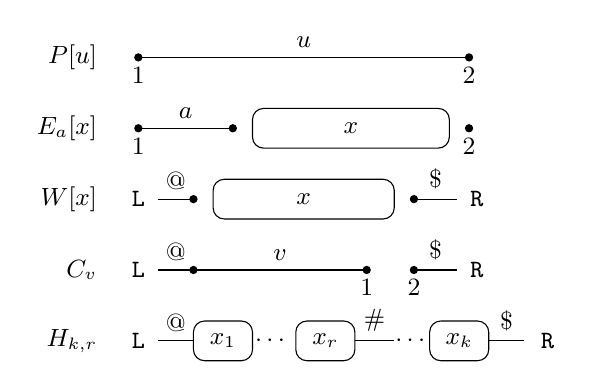
\begin{tikzpicture}[x=1.0cm,y=0.9cm,every node/.style={font=\small}]
  % P[u]
  \node[anchor=east] at (-0.4,4.0) {$P[u]$};
  \fill (0,4.0) circle (1.5pt); \fill (4.2,4.0) circle (1.5pt);
  \draw (0,4.0)--(4.2,4.0);
  \node[above] at (2.1,4.0) {$u$};
  \node[below] at (0,4.0) {$1$}; \node[below] at (4.2,4.0) {$2$};

  % E_a[x]
  \node[anchor=east] at (-0.4,3.0) {$E_a[x]$};
  \fill (0,3.0) circle (1.5pt); \fill (1.2,3.0) circle (1.5pt); \fill (4.2,3.0) circle (1.5pt);
  \draw (0,3.0)--node[above] {$a$}(1.2,3.0);
  \draw[rounded corners] (1.45,2.72) rectangle (3.95,3.28);
  \node at (2.70,3.0) {$x$};
  \node[below] at (0,3.0) {$1$}; \node[below] at (4.2,3.0) {$2$};

  % W[x]
  \node[anchor=east] at (-0.4,2.0) {$W[x]$};
  \node at (0,2.0) {$\mathtt L$}; \fill (0.7,2.0) circle (1.5pt); \fill (3.5,2.0) circle (1.5pt); \node at (4.3,2.0) {$\mathtt R$};
  \draw (0.25,2.0)--node[above] {$@$}(0.7,2.0);
  \draw[rounded corners] (0.95,1.72) rectangle (3.25,2.28); \node at (2.1,2.0) {$x$};
  \draw (3.5,2.0)--node[above] {$\$$}(4.05,2.0);

  % C_v
  \node[anchor=east] at (-0.4,1.0) {$C_v$};
  \node at (0,1.0) {$\mathtt L$}; \fill (0.7,1.0) circle (1.5pt); \fill (2.9,1.0) circle (1.5pt);
  \fill (3.5,1.0) circle (1.5pt); \node at (4.3,1.0) {$\mathtt R$};
  \draw (0.25,1.0)--node[above] {$@$}(0.7,1.0);
  \draw (0.7,1.0)--node[above] {$v$}(2.9,1.0);
  \draw (3.5,1.0)--node[above] {$\$$}(4.05,1.0);
  \node[below] at (2.9,1.0) {$1$}; \node[below] at (3.5,1.0) {$2$};

  % H
  \node[anchor=east] at (-0.4,0.0) {$H_{k,r}$};
  \node at (0,0) {$\mathtt L$};
  \draw (0.25,0)--node[above] {$@$}(0.7,0);
  \draw[rounded corners] (0.7,-0.28) rectangle (1.45,0.28); \node at (1.075,0) {$x_1$};
  \node at (1.7,0) {$\cdots$};
  \draw[rounded corners] (2.0,-0.28) rectangle (2.75,0.28); \node at (2.375,0) {$x_r$};
  \draw (2.75,0)--node[above] {$\#$}(3.25,0);
  \node at (3.48,0) {$\cdots$};
  \draw[rounded corners] (3.7,-0.28) rectangle (4.45,0.28); \node at (4.075,0) {$x_k$};
  \draw (4.45,0)--node[above] {$\$$}(4.9,0); \node at (5.2,0) {$\mathtt R$};
\end{tikzpicture}
\caption{Schematic lower-bound gadgets. Boxes denote variable hyperedges;
numbered endpoints indicate ordered interfaces. Ordinary graph edges are
undirected; orientation of encoded words is carried by interface order.}
\label{fig:gadgets}
\end{figure}

\subsection{DFA simulation inside exact FICS syntax}

Let
\(A=(Q,\Sigma,\delta,q_0,F)\)
be an accessible partial DFA. Introduce a rank-two predicate \(Q_q\) for each
state \(q\in Q\). For every defined transition \(\delta(q,a)=q'\), add
\begin{equation}
\label{eq:dfa-transition}
Q_q(E_a[x])\leftarrow Q_{q'}(S_x).
\end{equation}
Whenever \(\delta(q,a)\in F\), add the fact
\begin{equation}
\label{eq:dfa-terminal}
Q_q(P[a])\leftarrow.
\end{equation}
Finally introduce a rank-zero start predicate \(p\) and
\begin{equation}
\label{eq:dfa-wrapper}
p(W[x])\leftarrow Q_{q_0}(S_x).
\end{equation}

\begin{lemma}[Syntactic validity of the automaton clauses]
Every clause in \(\Gamma_A\) is a fixed-interface clause in the sense of the
FICS syntax.  In \eqref{eq:dfa-transition} and \eqref{eq:dfa-wrapper}, the
unique head variable-hyperedge occurrence is paired with the unique body star
atom carrying the same variable label and rank; in \eqref{eq:dfa-terminal}
both sets are empty.
\end{lemma}

\begin{proof}
This is immediate from the explicit definitions of \(E_a[x]\), \(S_x\),
\(P[a]\), and \(W[x]\). The head/body variable-occurrence correspondence is
bijective and preserves the ordered rank-two interface.
\end{proof}

\begin{lemma}[DFA simulation]\label{lem:dfa-sim}
For every state \(q\) and every rank-two ground graph pattern \(K\),
\(\Gamma_A\models Q_q(K)\)
iff there is a nonempty word \(u\) such that
\(K\cong_\iota P[u] \quad\text{and}\quad \delta(q,u)\in F.\)
\end{lemma}

\begin{proof}
Induct on the length of a refutation. A fact applies exactly to a one-edge
path \(P[a]\) with \(\delta(q,a)\in F\). Otherwise the first clause must be a
transition clause, forcing
\(K\cong_\iota\Real(E_a[x],x:=K')\)
with \(\Gamma_A\models Q_{\delta(q,a)}(K')\). The induction hypothesis gives
\(K'\cong_\iota P[v]\).  By \eqref{eq:prefix-frame-binding},
\(K\cong_\iota P[av]\), and the automaton condition follows. The converse is the same induction read along the word.
\end{proof}

Consequently,
\(\Gamma_A\models p(G)\)
iff \(G\cong\widehat P[u]\) for a nonempty word \(u\) accepted from \(q_0\).

\subsection{Anchored contexts and FCP}

For a word \(v=a_1\cdots a_j\), define a rank-two context \(C_v\) on distinct
vertices
\(\ell,c_0,\ldots,c_j,y,r.\)
The vertices \(\ell,r\) have labels \(\mathtt L,\mathtt R\), respectively,
and all others have label \(\mathtt N\). The ordinary edges are
\(\{\ell,c_0\}\), labeled \(\mathtt{@}\), the path edges
\(\{c_{i-1},c_i\}\), labeled \(a_i\), and \(\{y,r\}\), labeled
\(\mathtt{\$}\). Its ordered interface is
\(\iota(C_v)=(c_j,y).\)
In particular, \(C_v\) contains no ordinary edge \(\{c_j,y\}\). Whenever the
composition is defined,
\begin{equation}
\label{eq:anchored-context-concatenation}
C_v\odot P[u]\cong\widehat P[vu].
\end{equation}

\begin{lemma}[No cross-component edge collision]
\label{lem:no-cross-edge-collision}
Let \(G\) and \(K\) be rank-two graphs with ordered interfaces
\(\iota(G)=(g_1,g_2), \qquad \iota(K)=(k_1,k_2),\)
and suppose \(G\odot K\) is defined in the sense of
\cite{ShoudaiEtAl2026}.  An ordinary edge of \(G\) and an ordinary edge of
\(K\) can have the same image in the glued graph only if they are the
respective edges joining the two interface vertices.  Consequently, if \(G\)
has no ordinary edge \(\{g_1,g_2\}\), then every ordinary edge of \(K\) has a
distinct surviving image in \(G\odot K\), and every non-interface vertex of
\(K\) survives as a distinct vertex.
\end{lemma}

\begin{proof}
Before gluing, take disjoint copies of \(G\) and \(K\).  The quotient
identifies only \(g_1\) with \(k_1\) and \(g_2\) with \(k_2\); no
non-interface vertex of one component is identified with a vertex of the
other component.  Hence an edge \(\{u,v\}\) of \(G\) and an edge
\(\{u',v'\}\) of \(K\) can acquire the same unordered pair of endpoints only
when both endpoints of each edge belong to the respective interfaces.  Since
the interfaces have rank two, this forces the two edges to be
\(\{g_1,g_2\}\) and \(\{k_1,k_2\}\), respectively.  The final assertions are
immediate.
\end{proof}

\begin{lemma}[Anchored suffix rigidity]\label{lem:suffix}
Suppose \(C_v\odot K\) is defined and
\(C_v\odot K\cong\widehat P[w].\)
Then there is a unique nonempty word \(u\) such that
\(w=vu \quad\text{and}\quad K\cong_\iota P[u].\)
\end{lemma}

\begin{proof}
The marked path \(\widehat P[w]\) contains exactly one vertex labeled
\(\mathtt L\), exactly one vertex labeled \(\mathtt R\), and unique incident
marker edges labeled \(\mathtt{@}\) and \(\mathtt{\$}\). Any isomorphism
therefore fixes the two marker ends and forces the entire context prefix
\(\ell,c_0,\ldots,c_j\)
to coincide with the initial segment labeled \(v\). Hence \(v\) is a prefix
of \(w\); write \(w=vu\).

The two components in \(C_v\odot K\) share only the two ordered interface
vertices. The marker labels \(\mathtt L,\mathtt R,\mathtt{@},\mathtt{\$}\)
are disjoint from the internal word labels, so no internal feature of \(K\)
can be confused with either external marker.  Since \(C_v\) has no ordinary
edge between its two interface vertices, Lemma~\ref{lem:no-cross-edge-collision}
shows that every ordinary edge of \(K\) survives distinctly in the composition
and every non-interface vertex of \(K\) survives as a distinct vertex.  Any
branch, chord, cycle, extra edge, or extra non-interface vertex in \(K\) would
therefore survive and make the result non-isomorphic to the simple marked path
\(\widehat P[w]\). Consequently \(K\) is exactly the remaining suffix path,
with its first and second interface vertices mapped to the left and right ends
of that suffix. Hence \(K\cong_\iota P[u]\). Uniqueness follows from the
uniqueness of the suffix after a fixed prefix.
\end{proof}

\subsection{Boundary exposure of anchored path residuals}

The learner of \cite{ShoudaiEtAl2026} constructs its residual set from valid
ordered boundary specifications in positive examples.  For the anchored path
contexts above, the inserted suffix path is recovered by one explicit
rank-two specification.

\begin{lemma}[Explicit exposure of an anchored path residual]
\label{lem:block-residual-exposure}
Let \(v\) be a word and let \(u=a_1\cdots a_h\) with \(h\ge1\).  Put
\(G_{v,u}=C_v\odot P[u]\cong\widehat P[vu].\)
Let \(t_0,t_1,\ldots,t_h\) be the vertices of the copy of \(P[u]\) inside
\(G_{v,u}\), in path order, where \(t_0\) and \(t_h\) are the two vertices
identified with the ordered interface of \(C_v\).  Define
\(\beta_u=(t_0,t_h)\)
and let
\(E_u^\partial = \{e\in E(P[u]): e\cap\{t_0,t_h\}\ne\varnothing\},\)
where the edges are understood as their copies in \(G_{v,u}\).  Then
\((\beta_u,E_u^\partial)\) is a valid ordered boundary specification in the
sense of Definition~2.5 of \cite{ShoudaiEtAl2026}, and
\[
\boxed{
K_{G_{v,u}}(\beta_u,E_u^\partial)
\cong_\iota P[u].
}
\]
Consequently, if \(G_{v,u}\) occurs in a positive sample \(D_n\) and
\(w\ge2\), then
\(\operatorname{BRep}_w(D_n)\)
contains a representation \(\sigma_{v,u}\) such that
\(\operatorname{can}(\sigma_{v,u})\cong_\iota P[u].\)
\end{lemma}

\begin{proof}
The only vertices shared by the anchored context \(C_v\) and the inserted
path \(P[u]\) are \(t_0\) and \(t_h\).  Every edge in
\(E_u^\partial\) is incident with one of these boundary vertices, so
\((\beta_u,E_u^\partial)\) is valid.

Suppose first that \(h\ge2\).  After deleting \(t_0\) and \(t_h\) from
\(G_{v,u}\), the vertices \(t_1,\ldots,t_{h-1}\) form one connected path
component.  The non-boundary endpoints of the edges in \(E_u^\partial\) lie
in this component, so the reachable set
\(I_{G_{v,u}}(\beta_u,E_u^\partial)\) of Definition~2.5 is exactly
\(\{t_1,\ldots,t_{h-1}\}.\)
The context edge immediately preceding \(t_0\) and the marker edge incident
with \(t_h\) are not in \(E_u^\partial\); after deletion of the boundary
vertices, their remaining context components are therefore not reachable from
the selected boundary edges.  Hence
\(K_{G_{v,u}}(\beta_u,E_u^\partial)\) contains precisely the vertices
\(t_0,\ldots,t_h\) and precisely the \(u\)-labeled path edges between them.

If \(h=1\), there are no interior vertices and
\(E_u^\partial\) consists of the single edge joining the two boundary
vertices, so the same conclusion is immediate.  The boundary order
\((t_0,t_h)\) agrees with the ordered interface of \(P[u]\).  Therefore
\(K_{G_{v,u}}(\beta_u,E_u^\partial)\cong_\iota P[u].\)

Algorithm~1 of \cite{ShoudaiEtAl2026} enumerates all valid ordered boundary
specifications of rank at most \(w\) arising from the positive graphs in
\(D_n\).  Since the present specification has rank two, it is included in
\(\operatorname{BRep}_w(D_n)\) whenever \(w\ge2\), and its canonical graph is
interface-isomorphic to \(P[u]\).
\end{proof}

\begin{lemma}[Explicit exposure of an anchored context]
\label{lem:anchored-context-exposure}
With the notation of Lemma~\ref{lem:block-residual-exposure}, let
\(E_{v}^{\partial} = \{e\in E(C_v):e\cap\{t_0,t_h\}\ne\varnothing\},\)
where the edges are understood as their copies in \(G_{v,u}\).  Then
\((\beta_u,E_v^{\partial})\) is a valid rank-two ordered boundary
specification and
\[
\boxed{
K_{G_{v,u}}(\beta_u,E_v^{\partial})
\cong_\iota C_v.
}
\]
Consequently, if \(G_{v,u}\) occurs in a positive sample \(D_n\) and
\(w\ge2\), then \(\operatorname{BRep}_w(D_n)\) contains a representation
\(\rho_{v,u}\) with
\(\operatorname{can}(\rho_{v,u})\cong_\iota C_v.\)
\end{lemma}

\begin{proof}
This is the same boundary-separation argument used in the proof of
Lemma~4.15 of \cite{ShoudaiEtAl2026}.  After deleting the two shared interface
vertices \(t_0,t_h\), the non-interface part of the copy of \(C_v\) is
disjoint from the non-interface part of the inserted path \(P[u]\).
The boundary edge set \(E_v^\partial\) selects precisely the components on the
\(C_v\)-side of the cut.  Definition~2.5 therefore reconstructs exactly the
canonical copy of \(C_v\), with the original interface order.  Algorithm~1
then includes this rank-two representation in \(\operatorname{BRep}_w(D_n)\).
\end{proof}

Let \(\mathbf 0\) denote the empty rank-zero ground graph pattern. Whenever
rank-zero composition is taken with \(\mathbf 0\), it leaves the other
rank-zero ground graph unchanged up to isomorphism.

\begin{proposition}[FCP-preserving automaton embedding]\label{prop:fcp-embed}
If \(A\) is accessible, then \((\Gamma_A,p)\) satisfies FCP in the sense of
\cite{ShoudaiEtAl2026}. Moreover,
\(|\Gamma_A|=O(|Q|),\)
with fixed finite alphabets, rank-two auxiliary predicates, bounded degree,
and a fixed finite family of local head frames.
\end{proposition}

\begin{proof}
For \(q\in Q\), choose an access word \(v_q\) with
\(\delta(q_0,v_q)=q\). Consider any rank-two ground graph pattern \(K\) for
which \(C_{v_q}\odot K\) is defined.

If \(\Gamma_A\models Q_q(K)\), Lemma~\ref{lem:dfa-sim} gives
\(K\cong_\iota P[u]\) and \(\delta(q,u)\in F\). Hence, by
\eqref{eq:anchored-context-concatenation},
\(C_{v_q}\odot K\cong\widehat P[v_qu]\)
and the start predicate accepts the composition.

Conversely, if
\(\Gamma_A\models p(C_{v_q}\odot K),\)
the start-language characterization gives
\(C_{v_q}\odot K\cong\widehat P[w]\) for an accepted word \(w\).
Lemma~\ref{lem:suffix} yields \(w=v_qu\) and \(K\cong_\iota P[u]\). Therefore
\(\delta(q,u)=\delta(q_0,v_qu)\in F,\)
and Lemma~\ref{lem:dfa-sim} gives \(\Gamma_A\models Q_q(K)\).
Thus \(C_{v_q}\) witnesses FCP for \(Q_q\). The start predicate is witnessed
by \(\mathbf 0\), since \(\mathbf 0\odot G\cong G\) for every rank-zero
ground graph \(G\).

There are at most \(|Q||\Sigma|\) transition clauses and at most
\(|Q||\Sigma|\) terminal facts, plus one wrapper clause. Since \(\Sigma\) is
fixed, the clause count is \(O(|Q|)\). All graph frames used above belong to a
fixed finite family independent of \(|Q|\).
\end{proof}

\subsection{\texorpdfstring{$r$-active realization with a length gate}{r-active realization with a length gate}}

Fix \(1\le r\le k\), \(h\ge1\), and
\[
D=2^h,
\qquad
A_D=\{[P[u]]_{\cong_\iota}:u\in\{0,1\}^h\}.
\]
Because ordered-interface isomorphism preserves the edge-label sequence,
\(|A_D|=D\).

Let
\(S\subseteq(\{0,1\}^h)^r\)
be arbitrary and define
\[
F_S=
\{u_1\cdots u_r:(u_1,\ldots,u_r)\notin S\}
\subseteq\{0,1\}^{rh}.
\]
When \(F_S\ne\varnothing\), apply the residual-compression lemma to obtain a
partial DFA with
\(O_r(D^r/\log D)\)
states. Extend its classification branch so that it recognizes
\(F_S\#\{0,1\}^*:\)
the fixed-length final residual is made nonaccepting and receives a
\(\#\)-transition to an accepting state \(T\), and \(T\) loops on \(0,1\).
If \(F_S=\varnothing\), use a constant-size rejecting classification branch;
if \(F_S=\{0,1\}^{rh}\), use the ordinary residual construction before the
separator extension.

To make the body support exact, add a fresh access symbol \(\mathtt b\) and a
length-gate chain
\(B_0,B_1,\ldots,B_h\)
with
\[
\delta(q_0,\mathtt b)=B_0,
\qquad
\delta(B_j,a)=B_{j+1}
\quad(0\le j<h,\ a\in\{0,1\}),
\]
where \(B_h\) is accepting and has no outgoing \(0,1\)-transition.  The gate
is disjoint from the classification branch.  Hence
\begin{equation}
\label{eq:exact-length-gate}
\boxed{
\Gamma\models Q_{B_0}(P[u])
\quad\Longleftrightarrow\quad
|u|=h.
}
\end{equation}
The chain adds only \(O(h)=O(\log D)\) states, which is negligible relative to
\(O_r(D^r/\log D)\) for the asymptotic lower bound.  The symbol \(\mathtt b\)
never occurs in candidate-head strings.

For \(r<k\), define the rank-zero head scaffold
\(H_{k,r}[x_1,\ldots,x_k]\) using neutral vertices
\(z_0,\ldots,z_r,z_r^+,z_{r+1},\ldots,z_k\)
and \(k\) variable hyperedges. For \(1\le i\le r\), the ports of \(x_i\) are
\((z_{i-1},z_i)\); the ports of \(x_{r+1}\) are
\((z_r^+,z_{r+1})\); and subsequent variables continue in series. Add the
ordinary separator edge \(\{z_r,z_r^+\}\) labeled \(\#\), together with the
external \(\mathtt L/\mathtt{@}\) and \(\mathtt R/\mathtt{\$}\) markers.
For \(r=k\), place the \(\#\)-edge after the final variable slot and before
the right marker. Then
\begin{equation}
\label{eq:lower-head-realization}
\Real(H_{k,r};x_i:=P[u_i])
\cong
\widehat P[u_1\cdots u_r\#u_{r+1}\cdots u_k]
\end{equation}
for \(r<k\), with the evident terminal-separator version when \(r=k\).

Define the live candidate
\begin{equation}
\label{eq:lower-bound-candidate}
\gamma_{k,r}^{(h)}:
p(H_{k,r}[x_1,\ldots,x_k])
\leftarrow
Q_{B_0}(S_{x_1}),\ldots,Q_{B_0}(S_{x_k}).
\end{equation}
Both \(p\) and \(Q_{B_0}\) are live: the length-gate branch itself supplies
accepted start graphs, and \(Q_{B_0}\) accepts every length-\(h\) binary path.

\begin{lemma}[Exact fixed-interface validity of the lower-bound candidate]
\label{lem:lower-syntax}
The candidate \(\gamma_{k,r}^{(h)}\) is a fixed-interface clause with exactly
\(k\) distinct rank-two variable labels.  Its \(k\) head
variable-hyperedge occurrences are in bijection with the \(k\) body star
atoms, and the corresponding occurrence and star carry the same label and
ordered rank-two interface.
\end{lemma}

\begin{proof}
Each variable hyperedge \(x_i\) occurs exactly once in \(H_{k,r}\).  The body
contains exactly one star \(S_{x_i}\), which has no ordinary edge, one
variable hyperedge labeled \(x_i\), and interface equal to its ordered ports.
Thus the occurrence-to-body-star correspondence is
\(h_i\longleftrightarrow Q_{B_0}(S_{x_i}), \qquad 1\le i\le k,\)
a bijection preserving label and rank.  This is precisely the
occurrence-based fixed-interface condition; distinct substitution labels index
the product arity separately.
\end{proof}

For \(S\subseteq(\{0,1\}^h)^r\), write
\(S^\sharp = \{(P[u_1],\ldots,P[u_r]):(u_1,\ldots,u_r)\in S\}.\)

\begin{lemma}[Exact support of the lower-bound relation]
\label{lem:exact-support}
For the length-gated construction,
\[
\boxed{
V_{\Gamma_{D,S}^{(r)},\gamma_{k,r}^{(h)}}
=
S^\sharp\times A_D^{k-r}.
}
\]
In particular the rejection relation vanishes outside \(A_D^k\).
\end{lemma}

\begin{proof}
If some coordinate \(K_i\) is not a length-\(h\) binary path in \(A_D\), the
corresponding body atom \(Q_{B_0}(S_{x_i})\) is not refutable, by the exact
length gate, so the tuple is not rejected.  If every coordinate is
\(P[u_i]\) with \(|u_i|=h\), all body atoms are refutable.  By the separator
construction in \eqref{eq:lower-head-realization}, the head belongs to the
classification language exactly
when \(u_1\cdots u_r\in F_S\), i.e. exactly when
\((u_1,\ldots,u_r)\notin S\).  The body-positive/head-negative convention
therefore labels precisely the tuples in \(S^\sharp\times A_D^{k-r}\).
\end{proof}

\begin{lemma}[Context compatibility of the extremal box]
\label{lem:extremal-box-compatible}
For every lower-bound target/candidate pair
\((\Gamma_{D,S}^{(r)},\gamma_{k,r}^{(h)})\), choose
\(C_{\mathtt b}\) as the FCP context of the length-gate predicate
\(Q_{B_0}\), and choose the empty rank-zero context \(\mathbf 0\) for the
start predicate.  Then
\[
\boxed{
A_D^k
\subseteq
\Omega_{\Gamma_{D,S}^{(r)},\gamma_{k,r}^{(h)},C}.
}
\]
\end{lemma}

\begin{proof}
Take \((K_1,\ldots,K_k)\in A_D^k\), so
\(K_i=P[u_i]\) with \(|u_i|=h\).  Each body star realizes to
\(P[u_i]\).  The access-word construction for the gate state gives the
context \(C_{\mathtt b}\); its interface labels agree with those of
\(P[u_i]\), and it has no ordinary edge joining its two interface vertices.
Hence \(C_{\mathtt b}\odot P[u_i]\) is defined and equals the marked path
\(\widehat P[\mathtt b u_i]\) up to isomorphism.  The realized head has rank
zero, and composition with the empty rank-zero context \(\mathbf 0\) is
always defined.  Thus all realized body and head arguments satisfy the
compatibility conditions in the definition of \(\Omega\).
\end{proof}

\begin{theorem}[Uniform rich-regime realization]
\label{prop:fiber-real}
For every fixed \(k\ge2\), there exists one bounded FICS regime
\(\mathfrak B_k\) such that, simultaneously for every \(1\le r\le k\), all
sufficiently large powers of two \(D=2^h\), and every
\(S\subseteq(\{0,1\}^h)^r\) (equivalently, every
\(S^\sharp\subseteq A_D^r\)), there exist an FCP-FICS \(\Gamma_{D,S}^{(r)}\in\mathfrak B_k\) and a \emph{live}
admissible candidate \(\gamma_{k,r}^{(h)}\) with exactly \(k\) distinct
rank-two variable labels satisfying
\[
|\Gamma_{D,S}^{(r)}|
\le
C_{k,r}\frac{D^r}{\log D},
\]
and
\[
V_{\Gamma_{D,S}^{(r)},\gamma_{k,r}^{(h)}}
=
S^\sharp\times A_D^{k-r}.
\]
More explicitly, one may take
\[
\Delta=2,\qquad s=t=k,\qquad w=2,
\]
choose a constant \(d=d_k\), and fix one finite admissible head-frame family
\(\mathcal H_{d_k}\) containing every frame type used by the construction.
The choices \(d_k\), \(\Sigma_{V,k}\), \(\Sigma_{E,k}\), and
\(\mathcal H_{d_k}\) depend only on \(k\), not on \(r,D,S\), or \(m\).
\end{theorem}

\begin{proof}
The residual classifier uses \(O_r(D^r/\log D)\) states and the length gate
adds only \(O(\log D)\) states. Proposition~\ref{prop:fcp-embed} gives linear
clause overhead.  For fixed \(k\), let \(\mathcal H_{d_k}\) contain the
finitely many head-frame types used by the transition clauses, terminal facts,
wrapper and gate clauses, together with the candidate scaffolds
\(H_{k,1},\ldots,H_{k,k}\).  Choose \(d_k\) large enough to bound the vertex
degree of every one of these finitely many local frames, take \(s=t=k\) and
\(w=2\), and fix the finite alphabets used in the construction.  Every graph
generated by the start predicate is an externally marked path of maximum
ordinary degree two, so the semantic degree bound may be fixed as
\(\Delta=2\).  Hence every target and candidate used here satisfies the same
bounded parameters of Definition~2.25 of \cite{ShoudaiEtAl2026}, independently
of \(r,D,S,m\), and all targets lie in one fixed presentation-level subregime
\(\mathfrak B_k\) of
\(\mathcal{FICSL}^{\mathrm{FCP}}_{2}(m,k,k,2,d_k).\)
Lemma~\ref{lem:exact-support} gives the claimed exact relation.
\end{proof}

\begin{remark}[Dependence of hidden constants]
The present theorem fixes \(k\) and \(r\); no uniformity in growing \(k\) is
claimed.  The finite-state part of the lower bound is explicit.  Since the
residual word length is \(L=rh\) and \(D=2^h\), the residual-compression lemma
uses fewer than
\(12\,\frac{D^r}{r\log_2 D}\)
states before the constant-size separator extension and the \(h+1\)-state
length gate.  The remaining lower-bound constants come from the fixed linear
DFA-to-FICS simulation and the finite \(k\)-dependent head-frame family.  The
upper-bound constants additionally depend on the number of admissible bounded
clause skeletons and variable-equality patterns in the chosen regime.
Determining useful uniform dependence on growing \(k\) is left to the joint
\((m,k)\) problem in Section~\ref{sec:discussion}.
\end{remark}

\begin{theorem}[Learner realization of the extremal box]
\label{thm:alg3-extremal}
For every target/candidate pair supplied by
Theorem~\ref{prop:fiber-real}, let \(C_{\mathtt b}\) be the FCP context for the
accessible gate state \(B_0\), obtained from the access word \(\mathtt b\).
Consider a learner stage \(n\) at which the current predicate basis \(F\)
contains a representative \(\rho_B\) with
\(\operatorname{can}(\rho_B)=C_{\mathtt b}.\)
The special rank-zero representation \(\rho_\emptyset\) is available to
Algorithm~3 by definition.

Under every complete positive presentation, there is an integer \(N_D\) such
that for every \(n\ge N_D\) the current residual set
\(R=\operatorname{BRep}_2(D_n)\)
contains representations \(\sigma_u\), one for every
\(u\in\{0,1\}^h\), satisfying
\(\operatorname{can}(\sigma_u)\cong_\iota P[u].\)
The same positive anchored examples also expose a representation of
\(C_{\mathtt b}\); hence every update stage \(n\ge N_D\) that occurs in the
learner run has a suitable \(\rho_B\in F\).  Consequently, at every such
update stage the representative translation
\[
\widetilde\gamma_{k,r}^{(h)}:
 p_{\rho_\emptyset}(H_{k,r})
 \leftarrow
 p_{\rho_B}(S_{x_1}),\ldots,p_{\rho_B}(S_{x_k})
\]
belongs to the bounded candidate set of Algorithm~3, and its Cartesian-product
search explicitly examines every tuple in \(A_D^k\).  The resulting
body-positive/head-negative rejection bits on that box are exactly
\(S^\sharp\times A_D^{k-r}.\)
For each labeling \(S\) there is such a target/candidate pair; the theorem does
not assert that one fixed target or one learner run realizes all labelings.
This is a conditional realization statement: it asserts the behavior of every
update stage occurring after \(N_D\), but does not assert the existence of such
an update stage.
\end{theorem}

\begin{proof}
The gate state \(B_0\) is accessible by \(\mathtt b\), so the anchored-context
construction used in Proposition~\ref{prop:fcp-embed} gives its FCP context
\(C_{\mathtt b}\).  For every \(u\in\{0,1\}^h\), the exact length gate gives
\(\Gamma_{D,S}^{(r)}\models Q_{B_0}(P[u]),\)
and hence FCP gives the positive start-language graph
\(G_u=C_{\mathtt b}\odot P[u] \cong\widehat P[\mathtt b u].\)
Because the set of these graphs is finite, a complete positive presentation
contains all of them from some stage \(N_D\) onward.  Algorithm~4 of
\cite{ShoudaiEtAl2026} recomputes
\(R=\operatorname{BRep}_2(D_n)\)
at every stage in the present regime.  Lemma~\ref{lem:block-residual-exposure}
therefore supplies, for every \(n\ge N_D\) and every \(u\in\{0,1\}^h\), a
residual representation \(\sigma_u\in R\) with
\(\operatorname{can}(\sigma_u)\cong_\iota P[u]\).  Applying
Lemma~\ref{lem:anchored-context-exposure} to any one of the same positive
graphs gives a representation of \(C_{\mathtt b}\) in
\(\operatorname{BRep}_2(D_n)\).  At an update stage Algorithm~4 resets
\(F=\operatorname{BRep}_2(D_n)\), so a suitable \(\rho_B\) then belongs to
\(F\).

At every update stage \(n\ge N_D\) that occurs in the learner run,
Theorem~\ref{thm:alg3-realization} and
Lemma~\ref{lem:lower-syntax} show directly from the bounded-candidate
construction of Algorithm~3 that
\(\widetilde\gamma_{k,r}^{(h)}\) is one of the enumerated candidates.
The Cartesian-product loop of Algorithm~3 ranges over all families in
\(R^{X(\gamma)}\), so the representations \(\sigma_u\) ensure that every
canonical tuple in \(A_D^k\) is explicitly tested.  By
Lemma~\ref{lem:extremal-box-compatible}, the entire box lies in the
context-compatible domain, and Theorem~\ref{thm:alg3-realization} identifies
the learner-side rejection bit with \(V_{\Gamma,\gamma}\) pointwise there.
Finally, Lemma~\ref{lem:exact-support} gives exactly
\(S^\sharp\times A_D^{k-r}.\)
\end{proof}

\begin{corollary}[Spuriousness of the extremal candidate]
For the length-gated lower-bound pair,
\(V_{\Gamma_{D,S}^{(r)},\gamma_{k,r}^{(h)}}=\varnothing \quad\Longleftrightarrow\quad S=\varnothing.\)
Thus, after representative and witness exposure, a nonempty \(S\) supplies
exactly the substitution geometry by which the corresponding learner
candidate is rejected as spurious.
\end{corollary}

\subsection{Sharp fiber profile and entropy}

\begin{theorem}[Sharp live and full profiles in one fixed rich regime]
\label{thm:sharp-profile}
For every fixed \(k\ge2\), the regime \(\mathfrak B_k\) of
Theorem~\ref{prop:fiber-real} satisfies, simultaneously for every
\(1\le r\le k\),
\[
\boxed{
d_{r,\mathrm{live}}^{\mathfrak B_k}(m)
=
\Theta_{k,r}\!\left((m\log(m+1))^{1/r}\right)
}
\]
and therefore also
\[
\boxed{
d_r^{\mathfrak B_k}(m)
=
\Theta_{k,r}\!\left((m\log(m+1))^{1/r}\right).
}
\]
In particular,
\[
\VCbox_k(\mathcal V_k^{\mathfrak B_k}(m))
=
\Theta_k\!\left((m\log(m+1))^{1/k}\right)
\]
and
\[
d_1^{\mathfrak B_k}(m)=\Theta_k(m\log(m+1)).
\]
\end{theorem}

\begin{proof}
The upper bound is Theorem~\ref{thm:fiber-upper}, applied to the fixed regime
\(\mathfrak B_k\). For the lower bound, Theorem~\ref{prop:fiber-real} uses live candidates and shatters
an \(r\)-box of side \(D\) using at most
\(C_{k,r}D^r/\log D\)
clauses. Choosing a power of two
\(D=\Theta_{k,r}((m\log(m+1))^{1/r})\)
with a sufficiently small implicit constant keeps the clause budget at most
\(m\), yielding the matching lower bound.
\end{proof}

\begin{corollary}[Sharp candidate-rejection entropy in the rich regime]
\label{cor:entropy-sharp}
For the same regime \(\mathfrak B_k\),
\[
\boxed{
\log_2|\mathcal V_{k,\mathrm{live}}^{\mathfrak B_k}(m)|
=
\Theta_k(m\log(m+1))
}
\]
and
\[
\boxed{
\log_2|\mathcal V_k^{\mathfrak B_k}(m)|
=
\Theta_k(m\log(m+1)).
}
\]
Consequently, for every \(1\le r\le k\),
\[
\log_2|\mathcal V_k^{\mathfrak B_k}(m)|
=
\Theta_{k,r}\bigl((d_r^{\mathfrak B_k}(m))^r\bigr).
\]
\end{corollary}

\begin{proof}
The upper bound is Proposition~\ref{prop:entropy-upper}. For the lower bound,
take \(r=k\) in the live lower bound of Theorem~\ref{thm:sharp-profile}: a box of side
\(\Omega_k((m\log(m+1))^{1/k})\) is shattered, hence the live concept class contains
\(2^{\Omega_k(m\log(m+1))}\) distinct restrictions.  This gives the live
lower bound, while the full-class lower bound follows by inclusion; the
universal entropy upper bound applies to both classes.
\end{proof}

\begin{corollary}[Unified information scale]
For every fixed \(1\le r\le k\), in the rich regime \(\mathfrak B_k\),
\[
\boxed{
(d_{r,\mathrm{live}}^{\mathfrak B_k}(m))^r
\asymp_{k,r}
\log_2|\mathcal V_{k,\mathrm{live}}^{\mathfrak B_k}(m)|
\asymp_k
m\log(m+1),
}
\]
and the same asymptotic scale holds for the full candidate class.
\end{corollary}

\begin{remark}
The word \emph{simultaneously} refers to the common ambient regime
\(\mathfrak B_k\). The extremal grammar-candidate pair need not be the same for
different \(r\). Our lower bound uses \(r\) active variables and \(k-r\)
semantically dummy variables.  Moreover, shattering varies the target FICS with
the labeling.  Thus the theorem is a class-level capacity statement, not a
claim that one fixed target or one learner run realizes every labeling.
\end{remark}


\subsection{Simultaneously sharp fixed-target profiles}
\label{subsec:simultaneous-fixed-target}

We now prove the fixed-target half of the two-level capacity theorem.
Unlike the global lower bound, this construction is not allowed to change the
target when the desired labeling changes.  Instead, one master FICS stores,
inside its predicate structure, a finite \emph{bank} of live classifiers for
every fiber dimension \(1\le r\le k\).  The candidate syntax then selects one
classifier from this bank through its head predicate.  This realizes every
labeling needed for the relevant shattered box while keeping the target fixed.

The construction is the mechanism behind the separation
\(m\log m \qquad\text{versus}\qquad \log m:\)
the former allows the target presentation itself to change with the labeling,
whereas the latter forces all labeling information to coexist inside one
bounded target.

Fix \(k\ge2\).  Let \(n\) be a sufficiently large integer and put
\(L=\lfloor\log_2 n\rfloor.\)
For \(1\le r\le k\), define
\[
h_r=\left\lfloor\frac{L}{r}\right\rfloor,
\qquad
D_r=2^{h_r},
\qquad
N_r=D_r^r=2^{r h_r},
\]
and
\(A_r = \{[P[u]]_{\cong_\iota}:u\in\{0,1\}^{h_r}\}.\)
For \(n\ge2^k\), every \(h_r\) is positive.  Writing
\(L=qr+s\) with \(0\le s<r\) gives
\(N_r=2^{L-s},\)
and therefore
\begin{equation}
\label{eq:Nr-scale}
\frac{n}{2^r}
<
2^{L-r+1}
\le
N_r
\le
2^L
\le
n.
\end{equation}
Thus \(N_r=\Theta_{k,r}(n)\) simultaneously for all \(1\le r\le k\).

\paragraph{A master accessible DFA.}
Use the fixed alphabet
\(\Sigma^\star = \{0,1,\#,\lambda,\alpha,\beta\}.\)
The symbols \(0,1,\#\) are used by candidate-head words, \(\lambda\) is a
private liveness symbol, and \(\alpha,\beta\) are used only for selector
prefixes.

For each \(r\) and each
\(S\subseteq(\{0,1\}^{h_r})^r,\)
create a classifier root \(q_{r,S}\).  From \(q_{r,S}\), place a complete
binary trie of depth \(r h_r\).  Thus the state reached by a binary prefix
\(z\in\{0,1\}^{\le r h_r}\) will be denoted \(q_{r,S,z}\), with
\(q_{r,S,\varepsilon}=q_{r,S}\), and
\(\delta(q_{r,S,z},a)=q_{r,S,za} \qquad (|z|<rh_r,\ a\in\{0,1\}).\)
Let
\[
F_{r,S}
=
\{u_1\cdots u_r:
(u_1,\ldots,u_r)\notin S\}
\subseteq\{0,1\}^{rh_r}.
\]
Add one accepting state \(T_{r,S}\), put
\(\delta(q_{r,S,z},\#)=T_{r,S} \qquad (z\in F_{r,S}),\)
and let \(T_{r,S}\) loop on \(0\) and \(1\).  Finally add
\(\delta(q_{r,S},\lambda)=T_{r,S}.\)
Consequently every classifier root is live, and for every
\(z\in\{0,1\}^{rh_r}\) and \(v\in\{0,1\}^\ast\),
\begin{equation}
\label{eq:bank-classifier}
\delta(q_{r,S},z\#v)\in F
\quad\Longleftrightarrow\quad
z\in F_{r,S}.
\end{equation}
The additional \(\lambda\)-branch does not affect
\eqref{eq:bank-classifier}.

For each \(r\), also create a length-gate root \(B_r=B_{r,0}\) and states
\(B_{r,0},B_{r,1},\ldots,B_{r,h_r},\)
with
\(\delta(B_{r,j},a)=B_{r,j+1} \qquad (0\le j<h_r,\ a\in\{0,1\}),\)
where \(B_{r,h_r}\) is accepting and has no outgoing \(0,1\)-transition.
Thus
\begin{equation}
\label{eq:bank-gate}
\delta(B_r,u)\in F
\quad\Longleftrightarrow\quad
u\in\{0,1\}^{h_r}.
\end{equation}

It remains to make all of these roots accessible from one start state.
Let
\[
\mathcal R_n
=
\{q_{r,S}:1\le r\le k,\ S\subseteq(\{0,1\}^{h_r})^r\}
\cup
\{B_r:1\le r\le k\}
\]
and put \(J_n=|\mathcal R_n|\).
Choose
\(d_n=\lceil\log_2 J_n\rceil\)
and inject \(\mathcal R_n\) into the fixed-length code set
\(\{\alpha,\beta\}^{d_n}\).
Build the complete \(\alpha/\beta\)-selector trie of depth \(d_n\) from a
new start state \(q_0^\star\), and identify the selected leaves with the
corresponding roots in \(\mathcal R_n\).  Unused leaves are left as dead
states.  Because all selector codewords have the same length, no selected
root is an internal selector state.  Every state in the resulting partial
DFA
\(A_n^\star=(Q_n^\star,\Sigma^\star,\delta_n^\star,q_0^\star,F_n^\star)\)
is accessible.

\begin{lemma}[Size of the master DFA]
\label{lem:master-dfa-size}
For fixed \(k\),
\[
|Q_n^\star|
=
O_k(n2^n).
\]
\end{lemma}

\begin{proof}
For fixed \(r\), there are \(2^{N_r}\) classifier roots.  A complete binary
trie of depth \(rh_r\) has
\(2^{rh_r+1}-1 = 2N_r-1\)
states, and each classifier uses one additional accepting state.  Hence the
classifier bank has at most
\[
\sum_{r=1}^k 2^{N_r}(2N_r+1)
\le
(2n+1)k2^n
=
O_k(n2^n)
\]
states by \eqref{eq:Nr-scale}.  Also
\(J_n = \sum_{r=1}^k2^{N_r}+k = O_k(2^n).\)
The complete selector trie has fewer than \(2^{d_n+1}\le4J_n\) states.
Finally the \(k\) length gates use only
\(\sum_{r=1}^k(h_r+1)=O_k(\log n)\)
states.  Combining the three bounds proves the claim.
\end{proof}

Let
\(\Gamma_n^\star=\Gamma_{A_n^\star}\)
be the FICS obtained from the automaton simulation of
Section~\ref{sec:lower}.  Since \(A_n^\star\) is accessible,
Proposition~\ref{prop:fcp-embed} gives FCP and, because the alphabet
\(\Sigma^\star\) is fixed,
\begin{equation}
\label{eq:master-fics-size}
|\Gamma_n^\star|
=
O_k(n2^n).
\end{equation}

\paragraph{Rank-two candidate scaffolds.}
For \(1\le r<k\), define a rank-two head pattern
\[
G_{k,r}[x_1,\ldots,x_k]
\]
using neutral vertices
\[
z_0,\ldots,z_r,z_r^+,z_{r+1},\ldots,z_k.
\]
For \(1\le i\le r\), let \(x_i\) have ports
\((z_{i-1},z_i)\); let \(x_{r+1}\) have ports
\((z_r^+,z_{r+1})\); and for \(i>r+1\), let \(x_i\) have ports
\((z_{i-1},z_i)\).  Add the single ordinary edge
\(\{z_r,z_r^+\}\) labeled \(\#\), and take the ordered interface to be
\(\iota(G_{k,r})=(z_0,z_k).\)
For \(r=k\), use neutral vertices
\[
z_0,\ldots,z_k,z_k^+,
\]
let \(x_i\) have ports \((z_{i-1},z_i)\), add the ordinary
\(\#\)-edge \(\{z_k,z_k^+\}\), and take interface
\(\iota(G_{k,k})=(z_0,z_k^+).\)
Then, for \(u_i\in\{0,1\}^\ast\),
\begin{equation}
\label{eq:ranktwo-scaffold-realization}
\Real(G_{k,r};x_i:=P[u_i])
\cong_\iota
\begin{cases}
P[u_1\cdots u_r\#u_{r+1}\cdots u_k],&r<k,\\[1mm]
P[u_1\cdots u_k\#],&r=k.
\end{cases}
\end{equation}

For every \(S\subseteq(\{0,1\}^{h_r})^r\), define
\begin{equation}
\label{eq:fixed-target-candidate}
\gamma_{r,S}:
Q_{q_{r,S}}(G_{k,r}[x_1,\ldots,x_k])
\leftarrow
Q_{B_r}(S_{x_1}),\ldots,Q_{B_r}(S_{x_k}).
\end{equation}

\begin{lemma}[Syntax and liveness of the bank candidates]
\label{lem:bank-candidate-syntax}
For fixed \(k\), all candidates \(\gamma_{r,S}\) are live admissible
fixed-interface clauses in one bounded regime independent of \(n,r,S\).
They have exactly \(k\) distinct rank-two variable labels.
\end{lemma}

\begin{proof}
Each \(G_{k,r}\) contains exactly one variable-hyperedge occurrence labeled
\(x_i\) for each \(1\le i\le k\), and the body of
\eqref{eq:fixed-target-candidate} contains exactly one star \(S_{x_i}\) with
the same label and rank.  Hence the occurrence-to-body-star correspondence
is the bijection
\(x_i\longleftrightarrow Q_{B_r}(S_{x_i}), \qquad 1\le i\le k,\)
so the exact fixed-interface condition is satisfied.

The head pattern has rank two, matching the rank-two predicate
\(Q_{q_{r,S}}\), and every body predicate \(Q_{B_r}\) also has rank two.
Thus one may take \(s=t=k\) and \(w=2\).  For fixed \(k\), choose a constant
\(d_k^\star\) and let the finite family \(\mathcal H_{d_k^\star}\) contain
\(\{G_{k,1},\ldots,G_{k,k}\}\)
together with the finitely many automaton frames \(E_a\), \(P[a]\), and \(W\)
for the fixed alphabet \(\Sigma^\star\).  Hence the bounded parameters and
head-frame family are independent of \(n,r,S\).

Finally, \(Q_{B_r}\) is live by \eqref{eq:bank-gate}.  Also
\(\delta(q_{r,S},\lambda)=T_{r,S}\in F_n^\star,\)
so Lemma~\ref{lem:dfa-sim} gives
\(\Gamma_n^\star\models Q_{q_{r,S}}(P[\lambda]).\)
Thus every predicate occurring in \(\gamma_{r,S}\) is live.
\end{proof}

Let \(\mathfrak B_k^\star\) be the fixed presentation-level subregime of the
bounded FICS class of \cite{ShoudaiEtAl2026} obtained by fixing the finite
alphabets of the master-automaton construction, taking
\(\Delta=2,\qquad s=t=k,\qquad w=2,\)
choosing \(d=d_k^\star\), and fixing the finite admissible head-frame family
\(\mathcal H_{d_k^\star}\) described above.  All these choices depend only on
\(k\), not on \(n,r,S\), or the eventual clause budget \(m\).  Then every
\(\Gamma_n^\star\) and every candidate \(\gamma_{r,S}\) lie in this same
subregime.

For
\(S\subseteq(\{0,1\}^{h_r})^r,\)
write
\[
S^\sharp
=
\{(P[u_1],\ldots,P[u_r]):
(u_1,\ldots,u_r)\in S\}
\subseteq A_r^r.
\]

\begin{lemma}[Exact fixed-target bank relation]
\label{lem:fixed-target-bank-relation}
For every \(1\le r\le k\) and every
\(S\subseteq(\{0,1\}^{h_r})^r\),
\[
\boxed{
V_{\Gamma_n^\star,\gamma_{r,S}}
=
S^\sharp\times A_r^{k-r}.
}
\]
For \(r=k\), the second factor is understood as a singleton empty product.
\end{lemma}

\begin{proof}
Let \(\bar K=(K_1,\ldots,K_k)\in\Gtwo^k\).
If some \(K_i\) is not interface-isomorphic to a binary path
\(P[u_i]\) of length \(h_r\), then Lemma~\ref{lem:dfa-sim} together with
\eqref{eq:bank-gate} gives
\(\Gamma_n^\star\not\models Q_{B_r}(K_i).\)
Hence not all body atoms are refutable and
\(V_{\Gamma_n^\star,\gamma_{r,S}}(\bar K)=0\).

Now suppose
\(K_i\cong_\iota P[u_i], \qquad u_i\in\{0,1\}^{h_r} \quad(1\le i\le k).\)
All body atoms are then refutable.  By
\eqref{eq:ranktwo-scaffold-realization}, the realized head is the rank-two
path whose word is
\[
w=
\begin{cases}
u_1\cdots u_r\#u_{r+1}\cdots u_k,&r<k,\\
u_1\cdots u_k\#,&r=k.
\end{cases}
\]
The word before the separator has length \(rh_r\).  By
\eqref{eq:bank-classifier} and Lemma~\ref{lem:dfa-sim},
\[
\Gamma_n^\star\models Q_{q_{r,S}}(P[w])
\quad\Longleftrightarrow\quad
u_1\cdots u_r\in F_{r,S}
\quad\Longleftrightarrow\quad
(u_1,\ldots,u_r)\notin S.
\]
The candidate-rejection convention is body-positive/head-negative.
Therefore the tuple is rejected exactly when
\((u_1,\ldots,u_r)\in S\), proving the displayed equality.
The private \(\lambda\)-transition cannot affect this calculation because
the candidate-head word begins with \(0\) or \(1\).
\end{proof}

\begin{lemma}[Context compatibility of the fixed-target boxes]
\label{lem:fixed-target-bank-compatible}
For each classifier root \(q_{r,S}\), let \(v_{r,S}\in\{\alpha,\beta\}^{d_n}\)
be its selector access word, and let \(v_r\) be the selector access word of
\(B_r\).  Use the anchored FCP contexts \(C_{v_{r,S}}\) and \(C_{v_r}\).
Then
\[
A_r^k
\subseteq
\Omega_{\Gamma_n^\star,\gamma_{r,S},C}.
\]
\end{lemma}

\begin{proof}
Take \(K_i=P[u_i]\in A_r\).  Every body star realizes to \(P[u_i]\).
The anchored context \(C_{v_r}\) has matching rank-two interface labels and
no ordinary edge joining its two interface vertices, so
\(C_{v_r}\odot P[u_i]\)
is defined.  The realized head in
\eqref{eq:ranktwo-scaffold-realization} is also a rank-two path, and the same
argument shows that
\(C_{v_{r,S}}\odot\Real(G_{k,r};x_i:=P[u_i])\)
is defined.  Thus all body and head compositions required in the definition
of \(\Omega_{\Gamma_n^\star,\gamma_{r,S},C}\) are defined.
\end{proof}

\begin{theorem}[Simultaneously sharp fixed-target profiles]
\label{thm:simultaneous-fixed-target}
For every fixed \(k\ge2\), the bounded regime
\(\mathfrak B_k^\star\) above has, for all sufficiently large clause budgets \(m\),
a target
\[
\Gamma_m^\star\in\mathfrak B_k^\star,
\qquad
|\Gamma_m^\star|\le m,
\]
such that simultaneously for every \(1\le r\le k\),
\[
\boxed{
d_r(\Gamma_m^\star)
=
\Theta_{k,r}
\!\left((\log(m+1))^{1/r}\right).
}
\]
The lower bounds already hold using live admissible candidates.  Moreover,
\[
\boxed{
\log_2|\mathcal V_k(\Gamma_m^\star)|
=
\Theta_k(\log(m+1)).
}
\]
Consequently, for every \(1\le r\le k\),
\[
\boxed{
(d_r(\Gamma_m^\star))^r
\asymp_{k,r}
\log_2|\mathcal V_k(\Gamma_m^\star)|
\asymp_k
\log(m+1).
}
\]
\end{theorem}

\begin{proof}
First work with the target \(\Gamma_n^\star\).
Fix \(r\).  If \(r<k\), choose any
\(a_r\in A_r^{k-r}\)
and fix the last \(k-r\) coordinates to \(a_r\); for \(r=k\), no coordinates
are fixed.  By Lemma~\ref{lem:fixed-target-bank-relation}, as
\(S\subseteq A_r^r\)
varies, the corresponding fiber restrictions of
\(V_{\Gamma_n^\star,\gamma_{r,S}}\) realize every subset of \(A_r^r\).
Hence
\(d_r(\Gamma_n^\star)\ge D_r.\)
Using \eqref{eq:Nr-scale},
\(d_r(\Gamma_n^\star)^r \ge D_r^r = N_r > \frac{n}{2^r}.\)
Thus, simultaneously for all \(r\),
\begin{equation}
\label{eq:fixed-target-lower-n}
d_r(\Gamma_n^\star)
=
\Omega_{k,r}(n^{1/r}).
\end{equation}

By Lemma~\ref{lem:master-dfa-size} and
Proposition~\ref{prop:fcp-embed}, there is a constant \(C_k\) such that
\(|\Gamma_n^\star| \le C_k n2^n\)
for all sufficiently large \(n\).  Define
\(B_n=\lceil C_k n2^n\rceil.\)
Then
\(\log_2 B_n = n+\log_2 n+O_k(1) = \Theta_k(n).\)
For an arbitrary sufficiently large budget \(m\), choose the largest \(n\)
such that \(B_n\le m\), and set
\(\Gamma_m^\star=\Gamma_n^\star.\)
Since
\(m<B_{n+1} = O_k((n+1)2^{n+1}),\)
we still have
\(n=\Theta_k(\log(m+1)).\)
Combining this with \eqref{eq:fixed-target-lower-n} gives
\(d_r(\Gamma_m^\star) = \Omega_{k,r} \!\left((\log(m+1))^{1/r}\right).\)
The matching upper bound is Proposition~\ref{prop:fixed-target}, applied to
the fixed regime \(\mathfrak B_k^\star\).  This proves the profile statement.

For the entropy lower bound, use \(r=1\).  Then
\(N_1=D_1\ge n/2.\)
The relations
\(V_{\Gamma_n^\star,\gamma_{1,S}} = S^\sharp\times A_1^{k-1}, \qquad S\subseteq A_1,\)
are pairwise distinct, so
\(|\mathcal V_k(\Gamma_n^\star)| \ge 2^{N_1} \ge 2^{n/2}.\)
Hence
\(\log_2|\mathcal V_k(\Gamma_m^\star)| = \Omega_k(\log(m+1)).\)
The fixed-target entropy upper bound in
Proposition~\ref{prop:fixed-target} gives the matching
\(O_k(\log(m+1))\) estimate.  The final displayed equivalence follows.
\end{proof}

\begin{corollary}[Learner-side realization inside one target]
\label{cor:single-target-learner-realization}
Fix the master target \(\Gamma_n^\star\).  There is a sample threshold \(N_n\)
such that, for every learner stage \(j\ge N_n\), the current residual set
contains, simultaneously for every \(1\le r\le k\) and every \(P[u]\in A_r\),
a representation \(\sigma_{r,u}\) satisfying
\(\operatorname{can}(\sigma_{r,u})\cong_\iota P[u].\)
Moreover, at every update stage \(j\ge N_n\) that occurs in the learner run,
the predicate basis \(F\) contains representatives whose canonical graphs are
the explicit anchored FCP contexts \(C_{v_r}\) and \(C_{v_{r,S}}\) for all
bank predicates used at the fixed master size \(n\).  Consequently, at every
such update stage, for every \(r\) and every \(S\subseteq A_r^r\), the
representative translation of \(\gamma_{r,S}\) is an actual bounded candidate
of Algorithm~3, its Cartesian-product loop tests every tuple in \(A_r^k\),
and the rejection bits
on that box are exactly
\(S^\sharp\times A_r^{k-r}.\)
This is again a conditional realization statement: no existence claim is made
for an update stage \(j\ge N_n\).
\end{corollary}

\begin{proof}
For every \(u\in\{0,1\}^{h_r}\),
\(\Gamma_n^\star\models Q_{B_r}(P[u]),\)
so the anchored FCP context \(C_{v_r}\) gives the positive start-language
graph \(C_{v_r}\odot P[u]\).  By
Lemma~\ref{lem:block-residual-exposure}, once these graphs have appeared in the
positive sample, \(\operatorname{BRep}_2(D_j)\) contains residual
representations whose canonical graphs are all members of \(A_r\).

The same positive graphs expose the gate contexts \(C_{v_r}\) themselves by
Lemma~\ref{lem:anchored-context-exposure}.  For every classifier root
\(q_{r,S}\), the private liveness transition gives
\(\Gamma_n^\star\models Q_{q_{r,S}}(P[\lambda]),\)
so \(C_{v_{r,S}}\odot P[\lambda]\) is also a positive start-language graph;
Lemma~\ref{lem:anchored-context-exposure} extracts the explicit context
\(C_{v_{r,S}}\) from it.  For fixed \(n\), there are only finitely many
indices \(r,S,u\), hence a complete positive presentation contains all these
positive anchored graphs from some common stage \(N_n\) onward.

Algorithm~4 sets
\(R=\operatorname{BRep}_2(D_j)\) at every stage.  At an update stage it
also resets \(F=\operatorname{BRep}_2(D_j)\).  Thus every update stage \(j\ge N_n\) that occurs in the learner run
simultaneously contains all required residual and predicate representations.  The entire box lies in the context-compatible domain by
Lemma~\ref{lem:fixed-target-bank-compatible}.  Theorem~\ref{thm:alg3-realization}
then identifies the non-fact Cartesian-product admission test of Algorithm~3
with the target-relative rejection bit on \(A_r^k\), and Lemma~\ref{lem:fixed-target-bank-relation} gives the
exact relation \(S^\sharp\times A_r^{k-r}\).
\end{proof}

\section{Discussion and Open Problems}
\label{sec:discussion}

The two sharp theorems identify distinct information levels of the same
target-induced candidate-rejection mechanism.  Globally, both the target
presentation and the target-relative candidate may vary, and the available
description space has logarithm \(\Theta(m\log m)\) in the rich regime.
Conditional on one fixed target, only target-relative candidate choice
remains, reducing the exact information scale to \(\Theta(\log m)\).  The
distinction is therefore not merely between two proof techniques but between
two different sources of information in the target-induced candidate class:
\[
\boxed{
(d_r^{\mathfrak B_k}(m))^r\asymp m\log(m+1)
}
\qquad\text{versus}\qquad
\boxed{
(d_r(\Gamma_m^\star))^r\asymp\log(m+1).
}
\]
Both scales are simultaneously sharp for all \(1\le r\le k\).

\subsection{Graph-language, presentation, and candidate-rejection complexity}

Previous FGS VC/PAC results analyze generated graph languages
\(L(\Gamma,p)\subseteq\mathcal G.\)
Our object lies at the level of candidate evaluation:
\(V_{\Gamma,\gamma}\subseteq\Gtwo^k\)
records simultaneous substitutions on which a target-relative candidate is
rejected.  Refutability makes this more than a purely syntactic relation, but
it remains presentation-relative: equivalent presentations of the same start
language need not induce the same candidate class.  Actual target clauses do
not contribute nontrivial relations, by Lemma~\ref{lem:target-zero}.

\subsection{Relation to the FICS candidate test}

The bridge in Theorem~\ref{thm:alg3-realization} is deliberately a
representative translation rather than a set inclusion.  Target predicates
and learner representative predicates are different syntactic alphabets.  At
a stage where the required representatives belong to the current predicate
basis \(F\), the bounded-candidate construction of Algorithm~3 in
\cite{ShoudaiEtAl2026} includes the translated fixed-interface clause in its
candidate set, while its non-fact Cartesian-product admission test evaluates
the residual-family rejection bit studied here.  For live target predicates, Lemmas~4.15 and 4.17 of
\cite{ShoudaiEtAl2026} give the corresponding representative-exposure
mechanism at sufficiently large characteristic update stages.  Conversely,
the learner may contain boundary representatives that do not correspond to
target predicates, so we do not identify the full sample-induced candidate
space with \(\mathcal V_k^{\mathfrak B}(m)\).

\paragraph{Three levels of candidate space.}
It is useful to keep three levels distinct.  First,
\(\mathcal V_k^{\mathfrak B}(m)\) is a global target-induced class in which
both the target presentation and an admissible candidate over its active
predicates may vary.  Second, \(\mathcal V_k(\Gamma)\) fixes the target and
varies only such target-induced candidates.  Third, at a concrete learner
stage, Algorithm~3 constructs candidates over the sample-dependent basis
\(F\cup\{\rho_\emptyset\}\).  This third space may be strictly larger because
\(F\) can contain boundary representatives unrelated to target predicates.

The present capacity theorems concern the first two levels.  The direct
realization results establish an embedding of the relevant live
target-induced candidates into the third level at stages where their
representatives have been exposed; they do not identify the three classes.
Determining the capacity of the full sample-induced learner-state candidate
space is a separate problem.

The extremal construction sharpens this connection.  For each prescribed
labeling \(S\), Lemma~\ref{lem:block-residual-exposure} gives an explicit
ordered-boundary specification that recovers every path block \(P[u]\) from
the positive anchored graph \(C_{\mathtt b}\odot P[u]\).  Hence the current
residual set eventually contains all block substitutions in the extremal box.
Theorem~\ref{thm:alg3-extremal} then supplies, at stages with the required
predicate representative, an actual Algorithm~3 candidate whose rejection
bits on that box are exactly \(S\).  Lemma~\ref{lem:extremal-box-compatible}
verifies that the whole box lies inside the domain on which the FCP observation
bridge is valid.  Shattering is obtained across the family of targets; it
would be incorrect to say that one fixed target or one learner run shatters
the box.
This stagewise realization is conditional: representative exposure guarantees
the required contents of \(R\) and, at a sufficiently late update stage, of
\(F\), but it does not by itself guarantee that such a post-threshold update
stage occurs.

\subsection{FCP terminology and tuple-based distributional learning}

Our FCP is the FICS finite context property of \cite{ShoudaiEtAl2026}.  The
strong/weak/very weak finite-context and finite-kernel hierarchy for string
grammars \cite{KanazawaYoshinaka2017} is conceptually related through the
distributional-learning tradition, but no formal identification is made here.
Likewise, tuple-based MCFG work studies multidimensional nonterminals and
substitutability \cite{Yoshinaka2011,ClarkYoshinaka2014}.  The present arity
\(|X(\gamma)|\) instead counts simultaneous independent substitution slots in
one candidate clause.  A systematic transfer between these two notions of
arity would be interesting, but is outside the present theorem package.

\subsection{Global versus fixed-target fiber profiles}

The global sharp theorem varies both the target \(\Gamma\) and the candidate
\(\gamma\).  For a single fixed target, Proposition~\ref{prop:fixed-target}
gives
\(d_r(\Gamma) = O((\log(m+1))^{1/r}).\)
This logarithmic scale is operationally closer to the family of candidate
tests available during one run on one target.

Theorem~\ref{thm:simultaneous-fixed-target} closes the sharp-order question:
there is one bounded target family \(\Gamma_m^\star\) for which
\(d_r(\Gamma_m^\star)^r = \Theta_{k,r}(\log(m+1))\)
simultaneously for every \(1\le r\le k\).  Thus the global and fixed-target
scales are both sharp, but at different information levels:
\[
(m\log m)^{1/r}
\qquad\text{versus}\qquad
(\log m)^{1/r}.
\]
The construction also shows that the fixed-target lower bounds can be
witnessed by live candidates and, at any update stage occurring after the
relevant representative-exposure threshold, by actual candidate tests inside
one learner run on the same target.  This is a conditional stagewise
realization statement, not an assertion that a post-threshold update stage
must occur.

What remains open is not simultaneous sharpness but the finer structure of
all possible fixed-target profile vectors.

\begin{problem}[Fixed-target profile-vector characterization]
Characterize, up to asymptotic equivalence or sharp inequalities, the vectors
\(\bigl(d_1(\Gamma),\ldots,d_k(\Gamma)\bigr)\)
that can arise from one bounded FCP-FICS target \(\Gamma\) of clause budget
\(m\).  In particular, what tradeoffs, if any, are forced between different
fiber dimensions beyond the coordinatewise bounds
\(d_r(\Gamma)^r=O(\log(m+1))?\)
\end{problem}

\subsection{Growing arity}

All asymptotics above fix \(k\).

\begin{problem}[Joint \(m,k\) dependence]
Determine explicit bounds for
\(d_r(m,k)\)
when the number of independent clause variables is allowed to grow with the
grammar.
\end{problem}

\subsection{Description length instead of clause count}

The clause-budget formulation assumes a fixed bounded-head regime. If arbitrary
head graphs are allowed, one clause can encode unbounded syntax.

\begin{problem}[Description-length complexity]
Let \(\|\Gamma\|\) charge for the entire encoded syntax of a FICS. Determine
the higher-arity VC profile as a function of \(\|\Gamma\|\), without fixing a
finite head-frame family in advance.
\end{problem}

An information-theoretic upper bound linear in the bit description length is
natural, but the sharp lower-order factors depend on the chosen encoding.

\subsection{Minimal interfaces}

The lower bound already uses only paths, rank-two substitution interfaces,
fixed finite alphabets, and maximum graph degree two.

\begin{problem}[Minimal interface rank]
Can the \(m\log(m+1)\) entropy lower bound be realized with rank-one interfaces,
or is rank two necessary for transmitting ordered finite-state information
through substitution?
\end{problem}

\subsection{Algorithmic consequences}

The present results are capacity bounds, not runtime or membership-query lower bounds.  The learner searches only the residual tuples exposed by the current positive sample, whose exposure rate is not controlled by the present VC analysis.

\begin{problem}[Clause-test compression]
Can the fiber profile be exploited to reduce the product search over
\(R^{X(\gamma)}\)
used to validate candidate clauses, for example by
constructing small witness sets, adaptive tests, or parameterized procedures
for systems with small realized fiber profiles?
\end{problem}

This would connect the combinatorial analysis directly back to the product
search in the FICS learning algorithm \cite{ShoudaiEtAl2026}.

\subsection{A possible general template}

The proof also suggests a broader mechanism that is not pursued as a theorem
here. Suppose a bounded clause formalism has at most
\(2^{O(m\log(m+1))}\) canonical descriptions at syntax budget \(m\), and can
realize an \(n\)-state finite automaton with \(O(n)\) syntactic overhead while
preserving the relevant observation semantics. The same counting-versus-
finite-state-realization argument suggests an \(r\)-th-root box-capacity scale
of order \((m\log(m+1))^{1/r}\). Determining natural hypotheses under which this
becomes a formal transfer theorem is left for future work.

\subsection{Conclusion}

The candidate test of the FICS learner carries a higher-arity geometry that is
not visible from the generated start language alone.  Its distinct variable
labels index an explicit Cartesian substitution search, and the pointwise
body-positive/head-negative outcomes of that search form the
candidate-rejection relations studied here.

The main structural conclusion is a separation between two sharp information
regimes.  Conditional on one target presentation of clause budget \(m\),
variation within the target-induced candidate class has only logarithmic
entropy, and this bound is simultaneously sharp in every fiber dimension:
\((d_r(\Gamma_m^\star))^r \asymp_{k,r} \log_2|\mathcal V_k(\Gamma_m^\star)| \asymp_k \log(m+1).\)
One master target attains these bounds for all \(1\le r\le k\) at once by
storing finite banks of live classifier predicates.

If the target presentation is also allowed to vary, the available information
increases to the global scale
\((d_r^{\mathfrak B_k}(m))^r \asymp \log_2|\mathcal V_k^{\mathfrak B_k}(m)| \asymp m\log(m+1).\)
Thus the global \(m\log m\) term reflects target-presentation information in
addition to candidate choice; it should not be interpreted as the amount of
variation available inside one fixed learner target.

These two capacity levels concern target-induced candidate classes.  They
should not be confused with the potentially larger sample-dependent candidate
space over the learner basis \(F\).  Our Algorithm~3 realization results show
that the relevant live target-induced candidates occur inside that learner
space once their representatives have been exposed, but no capacity
characterization of the full learner-state space is claimed here.

Attaining both sharp scales inside the FICS framework requires an explicit
realization architecture: fixed-length residual compression, linear-size
partial-DFA simulation, preservation of FCP, live predicates, exact length
gates, anchored contexts, ordered-boundary residual exposure, and translation
into the candidate syntax actually tested by Algorithm~3.  At any update stage
occurring after the required finite exposure threshold, the translated learner
candidate realizes the prescribed pointwise rejection test.  This learner-side
statement is conditional on the occurrence of such an update stage.

The resulting picture connects finite-state description complexity to graph
grammar learning not merely through an abstract counting analogy, but through
an exact transfer into the learner-compatible candidate geometry of bounded
fixed-interface clause systems.  Conceptually, it also gives a concrete
grammatical-inference realization of the product-space perspective motivating
higher-dimensional PAC\(_n\)-learning: the higher arity comes directly from the
learner's simultaneous substitution slots, while the claims established here
remain deliberately at the level of sharp shattering capacity rather than a
general PAC\(_n\) characterization.

% References are embedded directly below; no external .bib file is required.
\begin{thebibliography}{16}
\providecommand{\natexlab}[1]{#1}
\providecommand{\url}[1]{\texttt{#1}}
\expandafter\ifx\csname urlstyle\endcsname\relax
  \providecommand{\doi}[1]{doi: #1}\else
  \providecommand{\doi}{doi: \begingroup \urlstyle{rm}\Url}\fi

\bibitem[Chernikov and Towsner(2020)]{ChernikovTowsner2020}
Artem Chernikov and Henry Towsner.
\newblock Hypergraph regularity and higher arity {VC}-dimension.
\newblock \emph{arXiv preprint arXiv:2010.00726}, 2020.

\bibitem[Chernikov and Towsner(2025)]{ChernikovTowsner2025}
Artem Chernikov and Henry Towsner.
\newblock Higher-arity {PAC} learning, {VC} dimension and packing lemma.
\newblock \emph{arXiv preprint arXiv:2510.02420v2}, 2025.

\bibitem[Clark and Yoshinaka(2014)]{ClarkYoshinaka2014}
Alexander Clark and Ryo Yoshinaka.
\newblock Distributional learning of parallel multiple context-free grammars.
\newblock \emph{Machine Learning}, 96\penalty0 (1--2):\penalty0 5--31, 2014.
\newblock \doi{10.1007/s10994-013-5403-2}.

\bibitem[Coregliano and Malliaris(2024)]{CoreglianoMalliaris2024}
Leonardo~N. Coregliano and Maryanthe Malliaris.
\newblock High-arity {PAC} learning via exchangeability.
\newblock \emph{arXiv preprint arXiv:2402.14294v3}, 2024.

\bibitem[Coregliano and Malliaris(2025)]{CoreglianoMalliaris2025}
Leonardo~N. Coregliano and Maryanthe Malliaris.
\newblock A packing lemma for {VCN}$_k$-dimension and learning high-dimensional
  data.
\newblock \emph{arXiv preprint arXiv:2505.15688v1}, 2025.

\bibitem[Coregliano and Opich(2026)]{CoreglianoOpich2026}
Leonardo~N. Coregliano and William Opich.
\newblock High-arity sample compression, 2026.
\newblock arXiv:2605.12465v2.

\bibitem[Ishigami and Tani(1997)]{IshigamiTani1997}
Yoshiyasu Ishigami and Seiichi Tani.
\newblock {VC}-dimensions of finite automata and commutative finite automata
  with $k$ letters and $n$ states.
\newblock \emph{Discrete Applied Mathematics}, 74\penalty0 (2):\penalty0
  123--134, 1997.
\newblock \doi{10.1016/S0166-218X(96)00025-X}.

\bibitem[Kanazawa and Yoshinaka(2017)]{KanazawaYoshinaka2017}
Makoto Kanazawa and Ryo Yoshinaka.
\newblock The strong, weak, and very weak finite context and kernel properties.
\newblock In \emph{Language and Automata Theory and Applications}, volume 10168
  of \emph{Lecture Notes in Computer Science}, pages 77--88. Springer, 2017.
\newblock \doi{10.1007/978-3-319-53733-7_5}.

\bibitem[Kobayashi et~al.(2015)Kobayashi, Kuriyama, and
  Takeuchi]{KobayashiKuriyamaTakeuchi2015}
Munehiro Kobayashi, Takayuki Kuriyama, and Kota Takeuchi.
\newblock Higher dimensional {PAC}$_n$-learning.
\newblock \emph{Congressus Numerantium}, 223:\penalty0 227--236, 2015.

\bibitem[Malliaris(2025)]{Malliaris2025Remarks}
Maryanthe Malliaris.
\newblock Remarks on a recent preprint of Chernikov and Towsner.
\newblock \emph{arXiv preprint arXiv:2510.19665v1}, 2025.

\bibitem[Kuriyama(2026a)]{KuriyamaFixedMonoidCFG}
Takayuki Kuriyama.
\newblock Distributional learning of context-free languages under fixed
  finite-monoid typing.
\newblock \emph{arXiv preprint arXiv:1409.6247v4}, 2026.
\newblock \doi{10.48550/arXiv.1409.6247}.

\bibitem[Kuriyama(2026b)]{KuriyamaFixedObservationMCFG}
Takayuki Kuriyama.
\newblock Positive-data learning of fixed-observation linear {MCFG}s from
  working binary presentations.
\newblock \emph{arXiv preprint arXiv:2605.11644v2}, 2026.
\newblock \doi{10.48550/arXiv.2605.11644}.

\bibitem[Shoudai et~al.(2023)Shoudai, Matsumoto, Suzuki, Uchida, and
  Miyahara]{ShoudaiEtAl2023PACFGS}
Takayoshi Shoudai, Satoshi Matsumoto, Yusuke Suzuki, Tomoyuki Uchida, and
Tetsuhiro Miyahara.
\newblock Parameterized formal graph systems and their polynomial-time {PAC}
  learnability.
\newblock \emph{IEICE Transactions on Fundamentals of Electronics,
  Communications and Computer Sciences}, E106-A\penalty0 (6):\penalty0
  896--906, 2023.
\newblock \doi{10.1587/transfun.2022EAP1052}.

\bibitem[Shoudai et~al.(2026)Shoudai, Matsumoto, Suzuki, and
  Uchida]{ShoudaiEtAl2026}
Takayoshi Shoudai, Satoshi Matsumoto, Yusuke Suzuki, and Tomoyuki Uchida.
\newblock Distributional learning of graph languages generated by
  fixed-interface clause systems, 2026.
\newblock arXiv:2604.26333v2.

\bibitem[Takeuchi(2020)]{Takeuchi2020}
Kota Takeuchi.
\newblock On {VC}$_2$-dimension and learnability.
\newblock \emph{RIMS K\^{o}ky\^{u}roku}, 2170:\penalty0 73--78, 2020.

\bibitem[Yoshinaka(2011)]{Yoshinaka2011}
Ryo Yoshinaka.
\newblock Efficient learning of multiple context-free languages with
  multidimensional substitutability from positive data.
\newblock \emph{Theoretical Computer Science}, 412\penalty0 (19):\penalty0
  1821--1831, 2011.
\newblock \doi{10.1016/j.tcs.2010.12.058}.

\end{thebibliography}

\end{document}
